\documentclass{class/llncs}
\usepackage[margin=1.3in]{geometry}
% \addtolength{\topmargin}{-.2in}
% \addtolength{\topmargin}{-.2in}
\usepackage{amssymb}
\usepackage{amsmath}
%\usepackage{tabularx}
\usepackage[table]{xcolor}
\usepackage{color}
\usepackage{caption}
\usepackage{algorithm}
\usepackage{algorithmicx}
% \usepackage{algorithm2e}
\usepackage{graphicx}
\usepackage{pgfplots}
\usepackage{comment}
\usepackage{mathrsfs} 
\usepackage{subcaption}
\usepackage{threeparttable}
\usepackage{multirow}
\usepackage{array}
\usepackage{mathrsfs} 
\usepackage{booktabs}

\newtheorem{Theorem}{Theorem}
\newtheorem{Definition}{Definition}
\newtheorem{Observation}{Observation}


\title{Identity-Based Key Aggregate Cryptosystem from Multilinear Maps}
\begin{document}
% 
\author{}
\institute{}

% \author{Sikhar Patranabis and Debdeep Mukhopadhyay}
% \institute{Department of Computer Science and Engineering\\ Indian Institute of Technology Kharagpur
% \\\{sikhar.patranabis, debdeep\}@cse.iitkgp.ernet.in}
\maketitle
\toctitle{Lecture Notes in Computer Science}
\tocauthor{Authors' Instructions}


\begin{abstract}

The recent advent of cloud computing has made secure online data sharing a vital application with far reaching impact in various fields. In this paper, we provide a public-key based solution to the online access delegation problem in which a data owner owning $N$ classes of encrypted data, wishes to securely grant access to any subset $S$ of these data classes among a subset $\hat{S}$ of data users. Our proposed solution is a $O(\log N)$-way multilinear map-based \emph{key-aggregate cryptosystem}~(KAC) that supports access delegation to $N$ data classes among $N$ different users. Our constructions have short ciphertexts, and low overhead public and private system parameters comprising of $O(\log N)$ group elements. Access to any arbitrary subset of data classes is provided by a single low overhead \emph{aggregate key}, which is then securely broadcast among the target subset of users. The systems are fully collusion resistant against any number of colluding parties and are agnostic of pre-defined data hierarchies. We propose three different KAC constructions based on symmetric and asymmetric multilinear maps, with distinct security parameters and implementation trade-offs. Each of these constructions can be used to build identity-based online data sharing systems suitable for real life applications.\\  

\noindent{\textbf{Keywords:}} Identity-based Key-Aggregate Cryptoystem, Online Data Sharing, Multilinear Maps, Collusion-resistant
\end{abstract}

\section{Introduction}
\label{sec:Intro}

The advent of cloud computing and the Internet of Things (IoT) has led to a massive rise in the demand for online data storage and data sharing services. Two very important paradigms that any data sharing service provider must ensure are privacy and flexibility. Since online data almost always resides in shared environments (for instance, multiple virtual machines running on the same physical device), ensuring privacy is a non trivial task. Current technology for secure data sharing comes in two major flavors - trusting a third party auditor \cite{cryptoeprint:2009:579} or using the user's own key to encrypt her data \cite{chow2012dynamic}. Figure \ref{fig:intro} describes a realistic online data sharing set-up. Suppose a data owner stores multiple classes of encrypted data online with the intention of providing users decryption keys to one or more such ciphertext classes, based on their respective credentials. She might also wish to dynamically update the delegated access rights based on 
changes to the data/credibility issues. The challenge therefore is to provide her with a secure and efficient online data sharing scheme that allows updates to user access rights on the fly. 


A n\"{a}ive (and extremely inefficient) solution is to have a different decryption key for each ciphertext class, and share them accordingly with users via secured channels. A more efficient proposition is the key-aggregate encryption (KAC) scheme proposed in \cite{chu2014key} that combines the power of individual decryption keys, for ciphertext classes in a given subset, into a single key for that subset. This key is specific to the designated subset, meaning that it cannot be used to decrypt any ciphertext class outside that subset. KAC derives its roots from the seminal work by Boneh \textit{et.al.} \cite{boneh2005collusion} that allows broadcasting of data (encrypted by the same public key) among multiple users, each of whom possess their own private keys for decryption. Both these schemes make use of bilinear mappings on multiplicative cyclic groups. 

 
 \begin{figure}[!t]
\centering
\captionsetup{font=scriptsize}
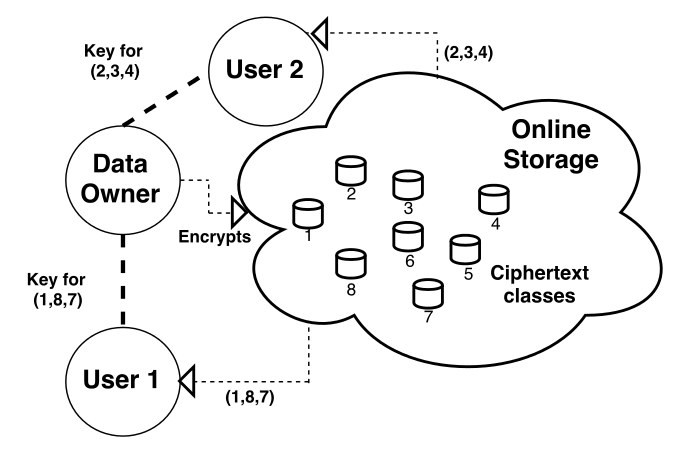
\includegraphics[scale=0.25]{Figs/KeyAgg.png}
\caption{Example of Online Data Sharing}
\label{fig:intro}
\end{figure}


\noindent{\textbf{Contributions:}} In this paper, we propose a basic key-aggregate scheme on additive elliptic subgroups that delegate decryption rights to multiple ciphertext classes using a single constant sized key. The scheme is dynamic in nature, that is, it allows the data owner to revoke access rights of users without having to change the entire set-up, unlike in the existing KAC scheme.  We then generalize this scheme into a two-level construction that allows flexible public key extension and maintains constant ciphertext size, while avoiding many of the pitfalls of earlier hierarchical schemes. We provide a formal proof of semantic security for the generalized scheme. We further extend the generalized scheme to allow using popular and efficiently implementable elliptic curve pairing schemes. We compare the time and space requirements of the proposed generalized scheme under various operating configurations. We also compare the performance of our proposed scheme, in terms of key size and resource 
utilization, with that of other existing schemes in literature.

\noindent{\textbf{Organization:}} The rest of the paper is organized as follows. Section \ref{sec:relwork} provides a brief overview of state of the art data sharing schemes. Section \ref{sec:prelims} introduces the notion of key aggregate cryptosystem, and provides a description of the complexity assumptions used to prove the semantic security of our proposed schemes. Our basic dynamic key-aggregate scheme is presented in Section \ref{sec:proposal}. We follow up with a more generalized two-tiered construction of the scheme for efficient public key extension in Section \ref{sec:general}, and prove its semantic security. A further extension for the generalized scheme that allows using efficiently implementable pairings is introduced and proved semantically secure in Section \ref{sec:extended}. Experimental results using Tate pairings based implementations of the extended scheme are presented in Section \ref{sec:results}. Finally Section \ref{sec:conclusions} concludes the paper.  



\section{Preliminaries}
\label{sec:prelims}

In this section, we formally define the key-aggregate cryptosystem~(KAC) framework as well its security. For clarity of understanding, we present the definition in two parts. The first part defines a basic KAC framework that focuses on generating small aggregate keys for arbitrarily large subsets of data classes. The second part extends this basic framework by combining it with broadcast encryption systems to distribute the aggregate key among multiple data users.

\subsection{Key-Aggregate Cryptosystem : The Basic Version}
\label{subsec:basic_framework}

The basic KAC is an ensemble of five poly-time randomized algorithms that are described next:\\

\noindent\textbf{SetUp}($\mathcal{ID}$): A data owner can classifying her data into one or more classes belonging an identity space $\mathcal{ID}$. The function sets up the key-aggregate cryptosystem for the identity space $\mathcal{ID}$. Outputs the public parameter $param$. \\

\noindent\textbf{KeyGen}(): Outputs a master-secret key $msk$ and the corresponding public key $PK$. A unique tuple $(msk,PK)$ is generated for each data owner.\\ 

\noindent\textbf{Encrypt}$(param,PK,i,\mathcal{M})$: Takes as input the public key parameter $PK$, the data class $i\in\mathcal{ID}$ and the plaintext message $\mathcal{M}$. Outputs the corresponding ciphertext $\mathcal{C}$, which is stored online in the shared environment.\\

\noindent\textbf{Extract}$(param,msk,\mathcal{S})$: Takes as input the master secret key and a polynomial size subset of data classes $\mathcal{S} \subseteq\mathcal{ID}$. Computes the aggregate key $K_{\mathcal{S}}$ for all encrypted data/messages classified into any class in $\mathcal{S}$.\\

\noindent\textbf{Decrypt}$(param,\mathcal{C},i,\mathcal{S},K_{\mathcal{S}})$: Takes as input the ciphertext $\mathcal{C}$, the data class $i$ and the aggregate key $K_{\mathcal{S}}$ corresponding to a subset $\mathcal{S}$. If $i\notin\mathcal{S}$, output $\bot$. Otherwise, outputs the decrypted message $\mathcal{M}$. The \textbf{Decrypt} function is invoked by a data user with the appropriate credentials to access one or more classes of data owned by the data owner. Note that the \textbf{Decrypt} operation for a given data user requires the explicit knowledge of the subset $\mathcal{S}$ of data classes that the corresponding user can access. This is of course a valid requirement since each user is expected to be aware of the subset $\mathcal{S}$ of data classes that she can access.

\subsubsection{Correctness.} For correctness, we require that the decryption algorithm always succeeds in decrypting a correctly encrypted plaintext message $m$. Formally, correctness of KAC may be described as follows. For any valid identity space $\mathcal{ID}$, any set $\mathcal{S}\subseteq\mathcal{ID}$, any index $i\in\mathcal{S}$, and any plaintext message $m$, we must have 
\begin{equation}
 Pr[\textbf{Decrypt}(\mathcal{C},i,\mathcal{S},K_{\mathcal{S}})=\mathcal{M} |\mathcal{E}]=1\nonumber
\end{equation}
where $\mathcal{E}$ is the event described as the conjunction of the following atomic events:
\begin{equation}
\begin{split}
param\leftarrow\textbf{SetUp}(\mathcal{ID}),(msk,PK)\leftarrow\textbf{KeyGen}(),\\
\mathcal{C}\leftarrow\textbf{Encrypt}(param,PK,i,\mathcal{M}),K_{\mathcal{S}}\leftarrow\textbf{Extract}(msk,\mathcal{S})\nonumber
\end{split} 
\end{equation}


\subsection{Security Definitions}
\label{subsec:security}

We define a formal framework for proving active chosen ciphertext security of KAC. We begin by introducing a game between a non-adaptive attack algorithm $\mathcal{A}$ and a challenger $\mathcal{B}$, both of whom are given $\mathcal{ID}$, the data class identity space, as input. The game proceeds through the following stages.\\
 
\noindent\textbf{SetUp}: Challenger $\mathcal{B}$ sets up the KAC system. In particular, $\mathcal{B}$ generates the public parameter $param$, the master secret key $msk$ and the public key $PK$. Of these, $param$ and $PK$ are furnished to $\mathcal{A}$.\\
 
\noindent\textbf{Query Phase 1}: Algorithm $\mathcal{A}$ adaptively issues decryption queries $q_1,\cdots,q_w$. Here a decryption query comprises of the tuple $(\mathcal{C},v)$, where $v\in\mathcal{ID}$ is the data class of the message encrypted as $\mathcal{C}$. The challenger has to respond a valid decryption of the ciphertext.\\
 
\noindent\textbf{Commit:} $\mathcal{A}$ adaptively commits to a set $\mathcal{S} \subset \mathcal{ID}$ of data classes that it wishes to attack. Since collusion attacks are allowed in our framework, $\mathcal{B}$ furnishes $\mathcal{A}$ with the aggregate key $K_{\overline{\mathcal{S}}}$ that allows $\mathcal{A}$ to decrypt any data class $v\notin\mathcal{S}$. Next, $\mathcal{B}$ randomly chooses a data class $i\in\mathcal{S}$ and provides it to $\mathcal{A}$.\\ 
 
\noindent\textbf{Challenge}: $\mathcal{A}$ picks at random two messages $\mathcal{M}_0$ and $\mathcal{M}_1$ from the set of possible plaintext messages and provides them to $\mathcal{B}$. To generate the challenge, $\mathcal{B}$ randomly picks $b\in\{0,1\}$, and sets the challenge to $\mathcal{A}$ as $(\mathcal{C}^{*},\mathcal{M}_0,\mathcal{M}_1)$, where ${\mathcal{C}}^{*}$ = \textbf{Encrypt}($PK,i,\mathcal{M}_b$).\\
 
\noindent\textbf{Query Phase 2}: $\mathcal{A}$ continues to adaptively issue decryption queries $q_{w+1},\cdots,q_{Q_D}$ where a decryption query comprises of the tuple $(\mathcal{C},v)$, but is now subject to the restriction $\mathcal{C}\neq {\mathcal{C}}^{*}$. $\mathcal{B}$ responds as in query phase 1.\\ 
 
 
\noindent\textbf{Guess}: $\mathcal{A}$ outputs a guess $b'$ of $b$. If $b' = b$, $\mathcal{A}$ wins the game.\\

% Note that the adversary $\mathcal{A}$ is non-adaptive; it chooses $\mathcal{S}$, and obtains the aggregate decryption key for all data classes outside of $\mathcal{S}$, before it even sees the public parameters $param$ or the public key $PK$

% \vspace{-2mm}
\noindent The game above models an attack in the real world setting where users who do not have authorized access to the subset $\mathcal{S}$ collude to try and expose a message in this subset. We now formally define the security notions for KAC. Let $Adv_{\mathcal{A},|\mathcal{ID}|}$ denote the probability that $\mathcal{A}$ wins the game.
\subsubsection{Definition 2.1.}
 A KAC construction is $(\epsilon,\mathcal{ID},Q_D)$ adaptively secure under a chosen ciphertext attack (that is, adaptively CCA-secure) if, for all adaptive probabilistic ploy-time algorithms $\mathcal{A}$ that can make a total of $Q_D$ decryption queries, we have that $|Adv_{\mathcal{A},|\mathcal{ID}|}-\frac{1}{2}| < \epsilon$.
 
\subsubsection{Definition 2.2.}
 A KAC construction is $(\epsilon,\mathcal{ID})$ adaptively secure under a chosen plaintext attack (that is, adaptively CPA-secure) if it is $(\epsilon,\mathcal{ID},0)$ adaptively CCA secure.\\


\noindent We also define two weaker notions of security in the non-adaptive setting. In particular, non-adaptive security is achieved in the scenario when $\mathcal{A}$ is required to commit to the set $\mathcal{S}$ before seeing the public parameters. We refer to such an adversary as a non-adaptive adversary. This leads to the following definitions.

\subsubsection{Definition 2.3.}
 A KAC construction is $(\epsilon,\mathcal{ID},Q_D)$ non-adaptively secure under a chosen ciphertext attack (that is, non-adaptively CCA-secure) if, for all non-adaptive probabilistic ploy-time algorithms $\mathcal{A}$ that can make a total of $Q_D$ decryption queries, we have that $|Adv_{\mathcal{A},|\mathcal{ID}|}-\frac{1}{2}| < \epsilon$.
% \end{Definition}

\subsubsection{Definition 2.4.}
 A KAC construction is $(\epsilon,\mathcal{ID})$ non-adaptively secure under a chosen plaintext attack (that is, non-adaptively CPA-secure) if it is $(\epsilon,\mathcal{ID},0)$ non-adaptively CCA secure.
% \end{Definition}

\subsection{Extensions to The Basic Version : Broadcasting Aggregate Keys}
\label{subsec:extensions}

We discuss in this paper two extensions to the basic framework of KAC for a full-fledged public key based implementation in practical data sharing environments. We first note that the standalone KAC framework presented in Section \ref{subsec:basic_framework} is a perfectly suitable choice when a single data owner wishes to delegate access rights to a particular subset of her data to a given data user. However, any practically deployable online data sharing scheme must be able to support multiple data owners, who should in turn be able to delegate access rights to their data to multiple users. In this context, there are two major requirements that the standalone KAC framework does not explicitly cater to:

\begin{itemize}
 \item Data privacy must be ensured for each individual data owner. In particular, an aggregate decryption key issued by one data owner should not leak information about the data of another data owner to an unauthorized user.
 \item Distribution of aggregate keys to a large number of data users must be handled efficiently and, preferably, via a public key based protocol and not a secure channel as suggested in \cite{chu2014key}.
\end{itemize}

\noindent In this paper, we augment the basic KAC framework to tackle both these problems efficiently. In particular, the second problem is handled by combining the basic KAC framework with that of the identity-based broadcast encryption scheme proposed in \cite{boneh2014low}. We formally define the combined scheme, referred to as the \emph{extended} KAC framework, using the following set of algorithms. Note that $\mathcal{ID}_1$ and $\mathcal{ID}_2$ denote the identity spaces for the data classes and the data users respectively.\\

\noindent\textbf{SetUp}($\mathcal{ID}_1,\mathcal{ID}_2$): Same as the basic KAC framework. \\

\noindent\textbf{OwnerKeyGen}(): In addition to the public key $PK$ and the master-secret key $msk$, also outputs a distribution-secret key $dsk$. The tuple $(msk,PK,dsk)$ is made available to the data owner.\\ 

\noindent\textbf{Encrypt}$(param,PK,dsk,i,\mathcal{M})$: Takes as input the data class $i\in\mathcal{ID}_1$ and the plaintext message $\mathcal{M}$. Outputs the corresponding ciphertext $\mathcal{C}$.\\

\noindent\textbf{UserKeyGen}$(param,msk,\hat{i})$: Takes as input the index $\hat{i}\in\mathcal{ID}_2$ for a user and outputs the corresponding secret key $d_{\hat{i}}$.\\ 

\noindent\textbf{Extract}$(param,msk,\mathcal{S})$: Takes as input the master secret key and a polynomial size subset of data classes $\mathcal{S} \subseteq\mathcal{ID}_1$. Computes the aggregate key $K_{\mathcal{S}}$ for all encrypted data/messages classified into any class in $\mathcal{S}$.\\

\noindent\textbf{Broadcast}$(param,K_{\mathcal{S}},\hat{\mathcal{S}},PK,dsk)$: Takes as input the aggregate key $K_{\mathcal{S}}$, the polynomial size target subset of users $\hat{\mathcal{S}}\subseteq\mathcal{ID}_2$. Outputs a single \emph{broadcast aggregate key} $K_{\left(\mathcal{S},\hat{\mathcal{S}}\right)}$ that allows any user $\hat{i}\in\hat{\mathcal{S}}$ to decrypt all encrypted data/messages classified into any class $i\in\mathcal{S}$.\\

\noindent\textbf{Decrypt}$(param,\mathcal{C},K_{\left(\mathcal{S},\hat{\mathcal{S}}\right)},i,\hat{i},d_{\hat{i}},\mathcal{S},\hat{\mathcal{S}})$: The decryption algorithm now takes, besides the ciphertext $\mathcal{C}$ and the corresponding data class $i\in\mathcal{S}$, a valid user id $\hat{i}\in\hat{\mathcal{S}}$. It also takes as input the broadcast aggregate key $K_{\left(\mathcal{S},\hat{\mathcal{S}}\right)}$ and the secret key $d_{\hat{i}}$. The algorithm outputs the decrypted message.\\

% \noindent We avoid presenting separately the game-based security framework for the extended KAC scheme here. The framework is directly introduced when proving the security of our proposed construction in Section \ref{subsec:multiuserKAC}.

\subsection{Security of Extended KAC: A Game Based Framework}
\label{subsec:gameextended}

We also define the formal framework for proving the security of the extended KAC via the following game between an attack algorithm $\mathcal{A}$ and a challenger $\mathcal{B}$:\\

\noindent\textbf{SetUp}: Challenger $\mathcal{B}$ sets up the KAC system. In particular, $\mathcal{B}$ generates the public parameter $param$, the master secret key $msk$, the distribution secret key $dsk$ and the public key $PK$. Of these, $param$ and $PK$ are furnished to $\mathcal{A}$.\\
 
\noindent\textbf{Query Phase 1}: Algorithm $\mathcal{A}$ adaptively issues decryption queries $q_1,\cdots,q_w$. Here a decryption query comprises of the tuple $(\mathcal{C},v)$, where $v\in\mathcal{ID}$ is the data class of the message encrypted as $\mathcal{C}$. The challenger has to respond a valid decryption of the ciphertext.\\
 
\noindent\textbf{Commit:} $\mathcal{A}$ adaptively commits to a set $\mathcal{S} \subset \mathcal{ID}_1$ of data classes and a corresponding set $\hat{\mathcal{S}} \subset \mathcal{ID}_2$ of authorized data users (with access to $\mathcal{S}$) that it wishes to attack. Since collusion attacks are allowed in our framework, $\mathcal{B}$ furnishes $\mathcal{A}$ with all the private user keys $d_{\hat{j}}$ for $\hat{j}\notin\hat{\mathcal{S}}$. In addition, $\mathcal{A}$ is also provided with the broadcast aggregate key $K_{\left(\overline{\mathcal{S}},\hat{\mathcal{S}}\right)}$ that allows any user in $\hat{\mathcal{S}}$ to decrypt any ciphertext class $v\notin{\mathcal{S}}$.\\  
 
\noindent\textbf{Challenge}: $\mathcal{A}$ picks at random two messages $\mathcal{M}_0$ and $\mathcal{M}_1$ from the set of possible plaintext messages and provides them to $\mathcal{B}$. To generate the challenge, $\mathcal{B}$ randomly picks $b\in\{0,1\}$, and sets the challenge to $\mathcal{A}$ as $(\mathcal{C}^{*},\mathcal{M}_0,\mathcal{M}_1)$, where ${\mathcal{C}}^{*}$ = \textbf{Encrypt}($PK,i,\mathcal{M}_b$).\\
 
\noindent\textbf{Query Phase 2}: $\mathcal{A}$ continues to adaptively issue decryption queries $q_{w+1},\cdots,q_{Q_D}$ where a decryption query comprises of the tuple $(\mathcal{C},v)$, but is now subject to the restriction $\mathcal{C}\neq {\mathcal{C}}^{*}$. $\mathcal{B}$ responds as in query phase 1.\\

\noindent\textbf{Guess}: $\mathcal{A}$ outputs a guess $b'$ of $b$. If $b' = b$, $\mathcal{A}$ wins the game.\\

The game above models an attack involving two different kinds of collusion. The first collusion is by all users not in $\hat{\mathcal{S}}$ who collude to try and expose an aggregate key that is broadcast for users in $\hat{\mathcal{S}}$ only. The second collusion is by users in $\hat{\mathcal{S}}$ who collude (by compromising the knowledge of the aggregate key for different subsets) to try and expose a message class in $\mathcal{S}$.

We next define the security of extended KAC. Let $Adv'_{\mathcal{A},|\mathcal{ID}_1|,|\mathcal{ID}_2|}$ denote the probability that $\mathcal{A}$ wins the above game.

\subsubsection{Definition 2.5.}
An extended KAC construction with the ability to broadcast aggregate keys is $(\epsilon,mathcal{ID}_1,\mathcal{ID}_2,Q_D)$ non-adaptively secure under a chosen ciphertext attack (that is, non-adaptively CCA-secure) if, for all non-adaptive probabilistic ploy-time algorithms $\mathcal{A}$ that can make a total of $Q_D$ decryption queries, we have that $|Adv'_{\mathcal{A},|\mathcal{ID}_1|,|\mathcal{ID}_2|}-\frac{1}{2}| < \epsilon$.
% \end{Definition}

\subsubsection{Definition 2.6.}
An extended KAC construction is $(\epsilon,\mathcal{ID}_1,\mathcal{ID}_2)$ non-adaptively secure under a chosen plaintext attack (that is, non-adaptively CPA-secure) if it is $(\epsilon,\mathcal{ID}_1,\mathcal{ID}_2,0)$ non-adaptively CCA secure.
 

\subsection{Multilinear Maps}
\label{subsec:multilinear}

In this section, we provide a brief overview of multilinear maps. Our description of multilinear maps is based on the \emph{graded encoding scheme} used in several candidate multilinear map constructions \cite{garg2013candidate}.

\subsubsection{Symmetric Multilinear Maps.} A standard symmetric multilinear map consists of the following pair of algorithms.\\

\noindent\textbf{SetUp}$'(1^\lambda,m)$: Sets up an $m$-linear map by outputting an $m$-tuple of groups $<\mathbb{G}_1,\mathbb{G}_2,\cdots,\mathbb{G}_m>$ of prime order $q$ (where $q$ is a $\lambda$ bit prime), along with the respective generator $g_i\in\mathbb{G}_i$ for $1\leq i\leq m$. In standard notation, $\mathbb{G}_1$ is the source group, $\mathbb{G}_m$ is the target group, and $\mathbb{G}_2,\cdots,\mathbb{G}_{m-1}$ are the intermediate groups.\\

\noindent$e_{i,j}(h_1,h_2)$: Takes as input $h_1\in\mathbb{G}_i$ and $h_2\in\mathbb{G}_j$, and outputs $h_3\in\mathbb{G}_{i+j}$ such that
\begin{equation}
 (h_1=g_i^a,h_2=g_j^b) \Rightarrow h_3=g_{i+j}^{ab}\nonumber
\end{equation}
\noindent In this paper, we follow the standard notation used in the literature to omit the subscripts and simply refer to this multilinear map as $e$. Further, $e$ may be generalized to multiple inputs as $e(h_1,\cdots,h_k)=e(h_1,e(h_2,\cdots,h_k))$. Note that $g^a_i$ is sometimes referred to as the level-$i$ \emph{encoding} of $a$. The scalar $a$ itself may therefore be referred to as the level $0$ encoding of itself.

\subsubsection{Asymmetric Multilinear Maps.} We adopt the same definition of asymmetric multilinear maps presented in \cite{garg2013candidate}. According to this definition, in asymmetric multilinear maps, the groups are indexed by integer vectors. Formally, a standard asymmetric multilinear map consists of the following algorithms.\\

\noindent\textbf{SetUp}$''(1^\lambda,\mathbf{m})$: Takes as input $\mathbf{m}\in\mathbb{Z}^l$. Sets up an $\mathbf{m}$-linear map by outputting an $m$-tuple of groups $<\mathbb{G}_{\mathbf{1}},\mathbb{G}_{\mathbf{2}},\cdots,\mathbb{G}_{\mathbf{m}}>$ of prime order $q$ (where $q$ is a $\lambda$ bit prime), along with the respective generator $g_{\mathbf{v}}\in\mathbb{G}_{\mathbf{v}}$ for $\mathbf{1}\leq \mathbf{v}\leq \mathbf{m}$(comparison is defined component-wise). Further, let $\mathbf{x}_i$ be the $i$th \emph{standard} basis vector (with $1$ at position $i$ and $0$ at each other position). In standard notation, $\mathbb{G}_{\mathbf{x}_i}$ is the $i$th source group, $\mathbb{G}_{\mathbf{v}}$ is the target group, and the rest are the intermediate groups.\\

\noindent$e_{\mathbf{i},\mathbf{j}}(h_1,h_2)$: Takes as input $h_1\in\mathbb{G}_\mathbf{i}$ and $h_2\in\mathbb{G}_\mathbf{j}$, and outputs $h_3\in\mathbb{G}_\mathbf{i+j}$ such that
\begin{equation}
 (h_1=g_\mathbf{i}^a,h_2=g_\mathbf{j}^b)\Rightarrow h_3=g_\mathbf{i+j}^{ab}\nonumber
\end{equation}
\noindent Again, we omit the subscripts and simply refer to this multilinear map as $e$, which may be generalized to multiple inputs as $e(h_1,\cdots,h_k)=e(h_1,e(h_2,\cdots,h_k))$.\\ 

In the forthcoming discussions, we present our KAC constructions assuming that the ideal multilinear maps based on the graded encoding scheme described above exist and are efficiently computable. We do this to make the analysis simple and easy to follow. We point out, however, that current candidates for multilinear maps in the cryptographic literature deviate from these ideal notions. In these candidates, group elements lack unique representations due to the presence of a noise term that tends to grow with repeated group/multilinear operations. However, as pointed out in \cite{boneh2014low}, most candidate constructions \cite{garg2013candidate,coron2013practical,gentry2014zeroizing,boneh2014immunizing} possess the necessary properties to instantiate public key constructions based on ideal multilinear maps. Unfortunately, most of these constructions have been cryptanalyzed \cite{cheon2015cryptanalysis,coron2014cryptanalysis}. To the best of our knowledge, the foremost candidate construction for multilinear maps currently unbroken is the graph-induced multilinear map based on lattices proposed by Gentry et al. \cite{gentry2015graph}, which naturally gives rise to asymmetric multilinear maps. We point out that it is possible to instantiate our KAC constructions using this candidate map since it meets our requirements listed below:

\let\labelitemi\labelitemii

\begin{itemize}
 \item The representation of an element should be statistically independent of the group and multilinear operations that led to that element. This is achieved using Kilian-style randomization \cite{kilian1988founding} on the encoding side \cite{gentry2015graph}.\\
 \item It is possible to extract a \emph{canonical} representation of an element in the target group given any representation of that element using the \emph{zero-test parameter}.\\
 \item The party setting up the multilinear map has sufficient \emph{trapdoor} information to compute $g^{\alpha^x}$ for a non-random $\alpha$ and exponentially large $x$.\\
 \item It is possible to generate asymmetric multilinear maps for any positive integer vector $\mathbf{m}\in\mathbb{Z}^l$.\\
%  \item It should be possible to design the parameters of our system such that the noise growth during the execution of our scheme does not lead to erroneous computations. 
\end{itemize}

\noindent However, in order to successfully instantiate our proposed schemes using graph induced multilinear map candidates, it is important to ensure that the algebraic elements used in our constructions are suitably encoded as paths in a directed graph and adequate precautions are taken to prevent weak trapdoor attacks.  

% We point out that the two foremost candidates for multilinear maps based on graded encoding schemes - the GGH candidate over ideal lattices \cite{garg2013candidate} and the CLT candidate over integers \cite{coron2013practical} would allow us to meet all these requirements. However, we also note that both these candidate constructions have been subjected to \emph{zeroizing attacks}\cite{cheon2015cryptanalysis}, also known as the weak discrete logarithmic attack. These attacks break the Subgroup Membership (SubM) and the decision linear (DLIN) problems on the GGH candidate map, and also completely break the CLT candidate. Initially it was conjectured that this attack could be thwarted by keeping the low-level encodings of $0$ private in the candidate constructions, and several fixes to these candidate constructions were provided based on this idea \cite{gentry2014zeroizing,boneh2014immunizing}. However, these extensions were also proven to be insecure in \cite{coron2014cryptanalysis}. 
% 
% In this paper, we propose using use the graph-induced multilinear map based on lattices proposed by Gentry et al. \cite{gentry2015graph} to instantiate our constructions. The graph-induced multilinear map, like the GGH and CLT candidate constructions, is also based on the graded encoding scheme and meets almost all the requirements listed above. The only significant drawback of this construction is the absence of the \emph{re-randomization} procedure (that helps to hide the group and multilinear operations leading to a particular element) to thwart cryptanalytic threats. However, a work around suggested in \cite{gentry2015graph} is to use Kilian-style randomization \cite{kilian1988founding} on the encoding side. This enhances the security of any scheme based on the graph induced candidate map, at the cost of some extra encoding bits.




% \noindent\textbf{The Multilinear Diffie-Hellman Exponent (MDHE) Assumption}:  Let $param\leftarrow SetUp'(n+l-1)$. Choose random 


 









\section{KAC Using Asymmetric Multilinear Maps}
\label{sec:proposal1}

In this section, we present the first construction of identity-based KAC based on asymmetric multilinear maps. Our construction is based on the basic KAC using bilinear pairings described in \cite{patranabis2015dynamic}. Their construction involves outputting a public parameter set consisting of $O(N)$ group elements, where $N$ is the number of data classes. Our goal in this scheme is to shrink the size of the public parameter to $O(\log N)$ group elements. To achieve this, we embed the original KAC scheme within a multilinear map, such that the original parameters can be derived from a small number of elements in the source group of the map. Hence it suffices to store these new elements as the public key of our proposed construction.

\subsubsection{The Basic Idea.} Let $N=2^m-1$ for some integer $m$, and let $\mathbf{m}$ be the $m+1$ length vector consisting of all ones. We use an asymmetric multilinear map with the target group $\mathbb{G}_{2\mathbf{m}}$. Note that if we pair two elements in the group $\mathbb{G}_{\mathbf{m}}$, we get an element in $\mathbb{G}_{2\mathbf{m}}$ by the definition of asymmetric multilinear maps. Let $Y_i=g^{\alpha^i}_{\mathbf{m}}$, where $\alpha\in\mathbb{Z}_q$. Recall that $\mathbf{x}_j$ is the $j$th \emph{standard} basis vector (with $1$ at position $j$ and $0$ at each other position) and $\mathbb{G}_{\mathbf{x}_j}$ is the $j$th source group with generator $g_{\mathbf{x}_i}$. Also, let $X_j=g^{\alpha^{(2^j)}}_{\mathbf{x}_j}$ for $0\leq j\leq m-1$ and $X_m=g^{\alpha^{(2^m+1)}}_{\mathbf{x}_m}$. We make the following claims.

\subsubsection{Claim 3.1.} Given an $i$ such that $0\leq i\leq N$, $Y_i$ can be computed from the set of parameters $(X_0,\cdots,X_m)$.
\subsubsection{Proof.} Let $i=\sum_{j=0}^{m-1}i_j2^j$. We have 
\begin{equation}
 Y_i=e(X^{i_0}_0g^{1-i_0}_{\mathbf{x}_0},\cdots,X^{i_{m-1}}_{m-1}g^{1-i_{m-1}}_{\mathbf{x}_{m-1}},g_{\mathbf{x}_m})\nonumber
\end{equation}
\subsubsection{Claim 3.2.} Given $i$ such that $N+2\leq i \leq 2N$, $Y_i$ can be computed from the set of parameters $(X_0,\cdots,X_m)$.
\subsubsection{Proof.} Let $i'=i-(2^m+1)=\sum_{j=0}^{m-1}i'_j2^j$. Then, we have  
\begin{equation}
 Y_i=e(X^{i'_0}_0g^{1-i'_0}_{\mathbf{x}_0},\cdots,X^{i'_{m-1}}_{m-1}g^{1-i'_{m-1}}_{\mathbf{x}_{m-1}},X_m)\nonumber
\end{equation}

\noindent We now make the following important observation.
\subsubsection{Observation 3.3.} \emph{Unless $g^{\alpha^{(2^m)}}_{\mathbf{x}_m}$ is published, it is difficult to compute the value of $Y_{N+1}$}.\\

\noindent This is the basic trick we use to embed a parameter set comprising of $O(N)$ group elements into another parameter set comprising of $O(\log N)$ group elements. We next present the construction of the basic single data-owner KAC using this framework.

\subsubsection{Assumption 3.4.} For simplicity, we assume in the forthcoming discussion that our plaintext messages are embedded as elements in the group $\mathbb{G}_{2\mathbf{m}}$. We discuss in Appendix \ref{app_sec:relaxation} how we may modify our scheme to relax this assumption.

\subsection{Construction for the Basic KAC Framework}
\label{subsec:construction}

We first present a basic construction for the KAC scheme assuming a single data owner and a single data user. The owner wishes to furnish the user with a \emph{single} low overhead aggregate key that allows the user to decryption rights to any data class $i\in\mathcal{S}$ where $\mathcal{S}$ is any arbitrary subset of $\{1,\cdots,N\}$. For the moment we assume that the aggregate key is received by the data owner from a trusted third party who sets up the overall system. We later show how this construction may be extended using public-key based broadcast encryption to distribute the aggregate key to multiple data users.   

Assume that \textbf{SetUp}$''(1^{\lambda},\mathbf{m})$ is the setup algorithm for an asymmetric multilinear map, where groups have prime order $q$ (where $q$ is a $\lambda$ bit prime) and $\mathbb{G}_{\mathbf{m}}$ is the target group. Our first basic identity-based KAC, for a single data owner with $N=2^m-1$ data classes, consists of the following algorithms.\\

\noindent\textbf{SetUp}$(1^{\lambda},m)$: Take as input the length $m$ of identities and the group order parameter $\lambda$. Set $\mathcal{ID}=\{0,1\}^m\backslash\{0\}^m$ as the identity space. Let $\mathbf{m}$ be the $m+1$ length vector consisting of all ones. Also, let $param''\leftarrow SetUp''(1^{\lambda},2\mathbf{m})$ be the public parameters for a multilinear map, with $\mathbb{G}_{2\mathbf{m}}$ being the target group. Choose a random $\alpha\in \mathbb{Z}_q$. Set $X_j=g^{\alpha^{(2^j)}}_{\mathbf{x}_j}$ for $0\leq j\leq m-1$ and $X_m=g^{\alpha^{(2^m+1)}}_{\mathbf{x}_m}$. Output the public parameter tuple $param$ as
\begin{equation}
 param = (param'',\{X_j\}_{j\in\{0,\cdots,m\}})\nonumber
\end{equation}
\noindent Discard $\alpha$ after $param$ has been output.\\

\noindent \textbf{KeyGen}(): Randomly pick $\gamma, t \in \mathbb{Z}_q$. Set the master secret key $msk$ to $(\gamma,t)$. Set the public key $PK=g^{\gamma}_{\mathbf{m}}$ and the user authentication key $U=g^{t}_{\mathbf{m}}$. Output the tuple $(msk,PK,U)$.\\

\noindent \textbf{Encrypt}$(params,PK,i,\mathcal{M})$: Take as input a message $\mathcal{M} \in \mathbb{G}_{2\mathbf{m}}$ belonging to class $i \in \mathcal{ID}$. Randomly choose $r\in\mathbb{Z}_q$ and let $t'=t+r \in\mathbb{Z}_q$. Recall that $Y_i=g^{\alpha^i}_{\mathbf{m}}$ and can be computed as per the formulation in Claim 3.1 for $1\leq i\leq N$. Output the ciphertext $\mathcal{C}$ as 
\begin{equation}
 \mathcal{C}=\left(g^r_{\mathbf{m}},(PK.Y_i)^{t'},\mathcal{M}.g^{t'\alpha^{(2^m)}}_{2\mathbf{m}}\right)\nonumber
\end{equation}
\noindent where $g^{t'\alpha^{(2^m)}}_{2\mathbf{m}}$ is computed as $\left(e(Y_{2^m-1},Y_1)\right)^{t'}$.\\

\noindent \textbf{Extract}$(params,msk,\mathcal{S})$: Let $msk=(msk_1,msk_2)$. For the input subset of data class indices $\mathcal{S}$, the aggregate key is computed as 
\begin{equation}
 K_{\mathcal{S}} = \prod_{v\in\mathcal{S}}Y^{msk_1}_{2^m-v}\nonumber
\end{equation} 
\noindent Note that this is indirectly equivalent to setting $K_{\mathcal{S}}$ to $\prod_{v\in\mathcal{S}}PK^{\alpha^{2^m-v}}$.\\
 
\noindent\textbf{Decrypt}$(params,\mathcal{C},i,\mathcal{S},K_{\mathcal{S}},U)$: If $i\notin\mathcal{S}$, output $\bot$. Otherwise, set
\begin{equation}
a_{\mathcal{S}}=\left(\prod_{v\in\mathcal{S},v\neq i}Y_{2^m-v+i}\right) \text{ and } b_{\mathcal{S}}=\left(\prod_{v\in\mathcal{S}}Y_{2^m-v}\right)\nonumber
\end{equation}
Let $\mathcal{C}=(c_0,c_1,c_2)$. Output the decrypted message as  
\begin{eqnarray} 
\hat{\mathcal{M}}&=&c_2\frac{{e}(K_{\mathcal{S}}.a_{\mathcal{S}},U.c_0)}{{e}(b_{\mathcal{S}},c_1)} \nonumber
\end{eqnarray}

\subsubsection{Correctness.} To see that the scheme is correct, that is, $\hat{\mathcal{M}}=\mathcal{M}$, put $c_0=g^r_{\mathbf{m}}$, $c_1=(PK.Y_i)^{t'}$ and $c_2=\mathcal{M}.g^{t\alpha^{(2^m)}}_{2\mathbf{m}}$. Then we have

\begin{equation}
\begin{split}
 \hat{\mathcal{M}}&=c_2\frac{{e}(K_{\mathcal{S}}.a_{\mathcal{S}},U.c_0)}{{e}(b_{\mathcal{S}},c_1)}\\
 &=c_2\frac{e(\prod_{v\in\mathcal{S}}Y^{\gamma}_{2^m-v}.\prod_{v\in\mathcal{S},v\neq i}Y_{2^m-v+i},g^{t'}_{\mathbf{m}})}{e(\prod_{v\in\mathcal{S}}Y_{2^m-v},(PK.Y_i)^{t'})}\\
 &=c_2\frac{e(\prod_{v\in\mathcal{S},v\neq i}Y_{2^m-v+i},g^{t'}_{\mathbf{m}})}{e(\prod_{v\in\mathcal{S}}Y_{2^m-v},Y_i^{t'})}\\
 &=\frac{\mathcal{M}.g^{t'\alpha^{(2^m)}}_{2\mathbf{m}}}{e(Y_{2^m},g^{t'}_{\mathbf{m}})}\\
 &=\mathcal{M}\nonumber
\end{split} 
\end{equation}

\subsubsection{Implementation Nuances.}  As stated in Section \ref{sec:prelims}, the only multilinear map candidate in the current literature that is not yet broken to the best of our knowledge is the graph-induced multilinear map construction proposed in \cite{gentry2015graph}. This graded-level encoding based construction contains noise terms that could lead to erroneous group operations, especially during repeated pairing computations. This could create complications, for example, in the computation of $g^{\alpha^{2^j}}_{\mathbf{x}_j}$ for sufficiently high values of $j$, especially if one attempts to compute it via level-0 encodings of random unknown $\alpha$. However, a work-around for this is to pre-compute the level-0 encodings for the various $\alpha^{2^j}$ (where $\alpha$ is known) and then pair them with the corresponding $g_{\mathbf{x}_j}$. This means that the system administrator must herself set up the multilinear map framework with the knowledge of the secret parameters used to set up the multilinear maps. Note, however, that the knowledge of these parameters is not required for either encryption and decryption, and hence may be discarded immediately after setup. Thus our KAC scheme may easily be instantiated by any noisy non-ideal candidate multilinear map without affecting the desired semantics in any way. Also note that the ciphertext and the aggregate key must not leak any important information, and hence need to be randomized appropriately. This implies that Kilian-style randomization parameters must be included for the group $\mathbb{G}_{\mathbb{m}}$. No other randomization parameters are necessary. We now look into the security of our proposed identity-based KAC construction.


\subsection{The Complexity Assumption}
\label{subsec:complexity}

We now briefly state the complexity assumption that is to be used to prove the security of the proposed KAC scheme. The assumption is introduced in \cite{boneh2014low}.

\subsubsection{The Hybrid Diffie-Hellman Exponent Assumption.} Let $param''$ is generated by \textbf{SetUp}$''(1^{\lambda},2\mathbf{m})$, where $\mathbf{m}$ is the $m+1$ length vector consisting of all ones. Choose $\alpha \in \mathbb{Z}_q$ at random (where $q$ is a $\lambda$-bit prime), and let $X_j=g^{\alpha^{(2^j)}}_{\mathbf{x}_j}$ for $0\leq j \leq m-1$. Also, define $X_m=g^{\alpha^{(2^m+1)}}_{\mathbf{x}_m}$. Choose a random $t'\in\mathbb{Z}_q$, and let $V=g^{t'}_{\mathbf{m}}$. The decisional $m$-Hybrid Diffie Hellman Exponent~(HDHE) problem as defined as follows. Given the tuple $(params'',\{X_j\}_{j\in\{0,\cdots,m\}},V,Z)$, distinguish if $Z$ is $g^{t'\alpha^{(2^m)}}_{2\mathbf{m}}$ or a random element of $\mathbb{G}_{2\mathbf{m}}$.

\subsubsection{Definition 3.5.} The decisional $m$-Hybrid Diffie-Hellman Exponent assumption holds for {SetUp}$''$ if, for any polynomial $m$ and a probabilistic poly-time algorithm $\mathcal{A}$, $\mathcal{A}$ has negligible advantage in solving the $m$-Hybrid Diffie-Hellman Exponent problem.

\subsection{Security of the Proposed KAC}
\label{subsec:security1}

We state and prove the non-adaptive CPA security of our proposed KAC scheme.

\subsubsection{Theorem 3.6.} \textit{Let \textbf{Setup}$''$ be the setup algorithm for an asymmetric multilinear map, and let the decisional $m$-Hybrid Diffie-Hellman Exponent assumption holds for {SetUp}$''$. Then our proposed basic KAC for $N$ data classes presented in Section \ref{subsec:construction} is non-adaptively CPA secure for $N=2^m-1$.}

\subsubsection{Proof.} Let $\mathcal{A}$ be a poly-time adversary such that $|Adv_{\mathcal{A},N}-\frac{1}{2}| > \epsilon$ for the proposed KAC system parameterized with an identity space $\mathcal{ID}$ of size $N=2^m-1$. Here $\epsilon$ is a non-negligible positive constant. We build an algorithm $\mathcal{B}$ that has advantage at least $\epsilon$ in solving the decisional $m$-HDHE problem for \textbf{Setup}$''$. $\mathcal{B}$ takes as input a random $m$-HDHE challenge $(params'',\{X_j\}_{j\in\{0,\cdots,m\}},V,Z)$ where:
\begin{itemize}
 \item $param''\leftarrow SetUp''(1^{\lambda},2\mathbf{m})$
 \item $X_j=g^{\alpha^{(2^j)}}_{\mathbf{x}_j}$ for $0\leq j \leq m-1$
 \item $X_m=g^{\alpha^{(2^m+1)}}_{\mathbf{x}_m}$
 \item $V=g^{t'}_{\mathbf{m}}$ for a random $t'\in\mathbb{Z}_q$ ($q$ being a $\lambda$ bit prime)
 \item $Z$ is either $g^{t'\alpha^{(2^m)}}_{2\mathbf{m}}$ or a random element of $\mathbb{G}_{2\mathbf{m}}$
\end{itemize}
\noindent $\mathcal{B}$ then proceeds as follows.\\

% \begin{enumerate}
\noindent \textbf{Commit:} $\mathcal{B}$ runs $\mathcal{A}$ and receives the set $\mathcal{S}$ of data classes that $\mathcal{A}$ wishes to be challenged on. $\mathcal{B}$ then randomly chooses a data class $i\in\mathcal{S}$ and provides it to $\mathcal{A}$.\\
 
\noindent \textbf{SetUp}: $\mathcal{B}$ should generate the public $param$, public key $PK$, the authentication key $U$, and the aggregate key $K_{\overline{\mathcal{S}}}$ and provide them to $\mathcal{A}$. They are generated as follows.
%  \vspace{-0.6mm}
\begin{itemize}
  \item $param$ is set as $(param'',\{X_j\}_{j\in\{0,\cdots,m\}})$.
  \item $PK$ is set as ${g^u_{\mathbf{m}}}/{Y_i}$ where $u$ is chosen uniformly at random from $\mathbb{Z}_q$ and $Y_i$ is computed as mentioned in Claim 3.1. 
  \item $U$ is set as $g^{t}_{\mathbf{m}}$ where $t$ is again chosen uniformly at random from $\mathbb{Z}_q$. Note that this is equivalent to setting $msk=((u-\alpha^i),t)$.
  \item $\mathcal{B}$ then computes   
  \begin{equation}
   K_{\overline{\mathcal{S}}} = \prod_{v\notin\mathcal{S}}\frac{Y^{u}_{2^m-v}}{Y_{2^m-v+i}}\nonumber
  \end{equation}
  \noindent Observe that $K_{\overline{\mathcal{S}}}=\prod_{v\notin\mathcal{S}}PK^{\alpha^{2^m-v}}$, as desired. Moreover, $\mathcal{B}$ is aware that $i\notin \overline{\mathcal{S}}$ (implying $i\neq v$), and hence has all the resources to compute $K_{\overline{\mathcal{S}}}$.  
\end{itemize}
 
\noindent Since the $g_{\mathbf{m}}$, $\alpha$, $u$, $t'$ and $t$ values are chosen uniformly at random, \emph{the public parameters and the public, private and authentication keys have an identical distribution to that in the actual construction}.\\
 
\noindent \textbf{Challenge}: $\mathcal{A}$ picks at random two messages $\mathcal{M}_0$ and $\mathcal{M}_1$ from the set of possible plaintext messages in $\mathbb{G}_{2\mathbf{m}}$, and provides them to $\mathcal{B}$. $\mathcal{B}$ randomly picks $b\in\{0,1\}$, and sets the challenge as $(\mathcal{C},\mathcal{M}_0,\mathcal{M}_1)$, where 
\begin{equation}
 \mathcal{C}=(U^{-1}V,V^u,\mathcal{M}_b.Z) \nonumber
\end{equation}
\noindent We claim that when $Z=g^{t\alpha^{(2^m)}}_{2\mathbf{m}}$ (i.e. the input to $\mathcal{B}$ is a valid $m$-HDHE tuple), then $(\mathcal{C},\mathcal{M}_0,\mathcal{M}_1)$ is a valid challenge to $\mathcal{A}$ as in a real attack. To see this, let $r=t'-t$. Then we have
\begin{eqnarray}
U^{-1}V=g^r_{\mathbf{m}}  &\text{ and }&  V^u= \left(g^u_{\mathbf{m}}\right)^{t'}=(PK.Y_i)^{t'}\nonumber \\
\mathcal{M}_b.Z&=&\mathcal{M}_b.g^{t'\alpha^{(2^m)}}_{2\mathbf{m}}\nonumber
\end{eqnarray}

\noindent Thus, by definition, $\mathcal{C}$ is a valid encryption of the message $\mathcal{M}_b$ in class $i$ and hence, $(\mathcal{C},\mathcal{M}_0,\mathcal{M}_1)$ is a valid challenge to $\mathcal{A}$. \\
 
\noindent \textbf{Guess}: The adversary $\mathcal{A}$ outputs a guess $b'$ of $b$. If $b' = b$, $\mathcal{B}$ outputs $0$ (indicating that $Z=g^{t'\alpha^{(2^m)}}_{2\mathbf{m}}$). Otherwise, it outputs $1$ (indicating that $Z$ is a random element in $\mathbb{G}_{2\mathbf{m}}$).\\ 

\noindent We conclude that $\mathcal{B}$ has the same advantage $\epsilon$ as $\mathcal{A}$, which must therefore be negligible, as desired. This completes the proof of Theorem 3.6. Note that this proof is in the standard model and does not use random oracles. \hfill\qed 

\subsubsection{CCA Security.} The CPA secure construction of Section \ref{subsec:construction} may be efficiently combined with a signature scheme to obtain a CCA secure construction. For details, refer Appendix \ref{app_sec:CCA1}.


\subsection{Extension to Multi-User Scenario}
\label{subsec:multiuserKAC}

We now generalize the KAC construction to a scenario where multiple data users wish to access a part of the data shared online by a single data owner. Assume that there are a maximum of $N_1$ data classes and and a maximum of $N_2$ users in the system. For simplicity, let $N_1=N_2=N$. The data owner grants access to a subset $\mathcal{S}$ of her data classes to a subset $\hat{\mathcal{S}}$ of the data users in the system. Here, both $\mathcal{S}$ and $\hat{\mathcal{S}}$ are arbitrary subset of $\{1,\cdots,N\}$, not necessarily equal. We show how the construction from Section \ref{subsec:construction} may be cleverly combined with the public-key based broadcast encryption scheme proposed in \cite{boneh2014low} to achieve a fully identity-based public key solution to this problem. 
% 
\subsubsection{Construction.} Let $N=2^m-1$ and $Setup''$ be as described before. The crux of the generalized scheme lies in the combination of the aggregate key with the broadcast encryption secret, although though they lie in different groups. Note that we do not need any additional parameters for incorporating broadcast encryption. Also note that generalization does not significantly blow up the overhead for any component of the system. In particular, the generalized scheme also consists of parameters that have size at most logarithmic in the number of data (and user) classes $N$. This allows $N$ to be exponentially large. Hence, the generalized system is fully identity-based with each data class and each user associated with a unique identity string $id\in\{0,1\}^{*}$. The class index $i$ and the user index $\hat{i}$ (where $1\leq i,\hat{i} \leq N$) are obtained by hashing the corresponding $id$ strings.\\\\
% 
\noindent\textbf{SetUp}$(1^{\lambda},m)$: Same as the construction in Section \ref{subsec:construction}.\\\\
% 
\noindent\textbf{OwnerKeyGen}(): Randomly pick $\gamma_1, \gamma_2, t \in \mathbb{Z}_q$. Set the master secret key $msk$ to $(\gamma_1,\gamma_2,t)$. Set $PK=(g^{\gamma_1}_{\mathbf{m}},g^{\gamma_2}_{\mathbf{m}})$ and $U=g^{t}_{\mathbf{m}}$. Output the tuple $(msk,PK,U)$.\\\\
% 
\noindent\textbf{Encrypt}$(params,PK,i,\mathcal{M})$: Take as input a message $\mathcal{M} \in \mathbb{G}_{2\mathbf{m}}$ belonging to class $i \in \mathcal{ID}$. Randomly choose $r\in\mathbb{Z}_q$ and let $t'=t+r \in\mathbb{Z}_q$. Recall that $Y_i=g^{\alpha^i}_{\mathbf{m}}$ and can be computed as per the formulation in Claim 3.1 for $1\leq i\leq N$. Also, let $PK=(PK_1,PK_2)$. Output the ciphertext $\mathcal{C}$ as 
\begin{equation}
 \mathcal{C}=\left(g^r_{\mathbf{m}},PK^r_1,(PK_1.Y_i)^{t'},\mathcal{M}.g^{t'\alpha^{(2^m)}}_{2\mathbf{m}}\right)\nonumber
\end{equation}
\noindent Note that the additional group element in the tuple blows up the ciphertext overhead by only a constant factor.\\

\noindent\textbf{UserKeyGen}$(params,msk,\hat{i})$: Let $msk=(msk_1,msk_2,msk_3)$. Output the secret key for data user $\hat{i}$ as \begin{equation}
 d_{\hat{i}}=Y^{msk_2}_{\hat{i}}\nonumber
\end{equation}

\noindent\textbf{Extract}$(params,msk,\mathcal{S},\hat{\mathcal{S}})$: The \textbf{Extract} operation now broadcasts the aggregate key $K_{\mathcal{S}}$ to all users in $\hat{\mathcal{S}}$ as follows. Let $msk=(msk_1,msk_2,msk_3)$. For the input subset of data class indices $\mathcal{S}$, compute $K_{\mathcal{S}} = \prod_{v\in\mathcal{S}}Y^{\gamma_1}_{2^m-v}$. Now, it is necessary to distribute this aggregate key to all users in $\hat{\mathcal{S}}$. For this, randomly choose $\hat{t}\in\mathbb{Z}_q$ and set $b_{\hat{\mathcal{S}}}=\left(\prod_{\hat{v}\in\hat{\mathcal{S}}}Y_{2^m-\hat{v}}\right)$. Output 
\begin{equation}
K_{\left(\mathcal{S},\hat{\mathcal{S}}\right)}=\left(g^{\hat{t}}_{\mathbf{m}},\left(g^{msk_2}_{\mathbf{m}}.b^{\hat{t}}_{\hat{\mathcal{S}}}\right),\mathcal{K}\right)\nonumber
\end{equation}
\noindent where 
\begin{equation}
\mathcal{K} = \left(\left(g^{\hat{t}\alpha^{(2^m)}}_{2\mathbf{m}}\right).\left(e(K_{\mathcal{S}},g^{msk_3}_{\mathbf{m}})\right)\right)\nonumber
\end{equation}
\noindent Note that the actual group element corresponding to $K_{\mathcal{S}}$ is difficult to recover from $\mathcal{K}$. However, as we demonstrate next, this knowledge is not explicitly necessary for decryption.\\\\
%  
\noindent\textbf{Decrypt}$(\mathcal{C},K_{\left(\mathcal{S},\hat{\mathcal{S}}\right)},i,\hat{i},d_{\hat{i}},\mathcal{S},\hat{\mathcal{S}},U)$: If $i\notin\mathcal{S}$ or $\hat{i}\notin\hat{\mathcal{S}}$, output $\bot$. Otherwise, set
\begin{eqnarray}
 a_{\hat{\mathcal{S}}}=\left(\prod_{\hat{v}\in\hat{\mathcal{S}},\hat{v}\neq \hat{i}}Y_{2^m-\hat{v}+\hat{i}}\right)&\text{ , }&
 a_{\mathcal{S}}=\left(\prod_{v\in\mathcal{S},v\neq i}Y_{2^m-v+i}\right)\nonumber\\ 
 \text{and }b_{\mathcal{S}}&=&\left(\prod_{v\in\mathcal{S}}Y_{2^m-v}\right)\nonumber
\end{eqnarray}
\noindent Let $\mathcal{C}=(c_0,c_1,c_2,c_3)$ and $K_{\left(\mathcal{S},\hat{\mathcal{S}}\right)}=(\hat{k}_0,\hat{k}_1,\hat{k}_2)$. Output the decrypted message as  
\begin{eqnarray} 
\hat{\mathcal{M}}&=&c_3.\hat{k}_2.\left(\frac{e(b_{\mathcal{S}},c_1){e}(a_{\mathcal{S}},U.c_0)}{{e}(b_{\mathcal{S}},c_2)}\right).\left(\frac{e(d_{\hat{i}}.a_{\hat{\mathcal{S}}},\hat{k}_0)}{e(Y_{\hat{i}},\hat{k}_1)}\right) \nonumber
\end{eqnarray}

\noindent Correctness of this scheme may be easily proven. We demonstrate next that this scheme is non-adaptively CPA secure in the standard model. We first describe the complexity assumption that is used to prove security. 

\subsubsection{The Extended Hybrid Diffie-Hellman Exponent Assumption.} Let $param''$ is generated by \textbf{SetUp}$''(1^{\lambda},2\mathbf{m})$, where $\mathbf{m}$ is the $m+1$ length vector consisting of all ones. Choose $\alpha \in \mathbb{Z}_q$ at random (where $q$ is a $\lambda$-bit prime), and let $X_j=g^{\alpha^{(2^j)}}_{\mathbf{x}_j}$ for $0\leq j \leq m-1$. Also, define $X_m=g^{\alpha^{(2^m+1)}}_{\mathbf{x}_m}$. Choose random $t',\hat{t}\in\mathbb{Z}_q$, and let $V_1=g^{t'}_{\mathbf{m}}$ and $V_2=g^{\hat{t}}_{\mathbf{m}}$. The decisional $m$-Extended Hybrid Diffie Hellman Exponent~(EHDHE) problem as defined as follows. Given the tuple
\begin{equation}
\left(params'',\{X_j\}_{j\in\{0,\cdots,m\}},(V_1,V_2),(Z_1,Z_2)\right)\nonumber
\end{equation}
\noindent distinguish if $(Z_1,Z_2)$ is $\left(g^{t'\alpha^{(2^m)}}_{2\mathbf{m}},g^{\hat{t}\alpha^{(2^m)}}_{2\mathbf{m}}\right)$ or a random element in $\mathbb{G}_{2\mathbf{m}}\times\mathbb{G}_{2\mathbf{m}}$.\\

\subsubsection{Definition 3.7.} The decisional $m$-EHDHE assumption holds for {SetUp}$''$ if, for any polynomial $m$ and a probabilistic poly-time algorithm $\mathcal{A}$, $\mathcal{A}$ has negligible advantage in solving the $m$-EHDHE problem.\\

It is not difficult to show that the $m$-EHDHE assumption holds for {SetUp}$''$ if the $m$-HDHE assumption holds for {SetUp}$''$.


\subsection{Security of the Multi-User Extension}
\label{subsec:security1_1}

We state and prove the non-adaptive CPA security of the extended multi-user KAC.

\subsubsection{Theorem 3.8.} \textit{Let \textbf{Setup}$''$ be the setup algorithm for an asymmetric multilinear map, and let the decisional $m$-EHDHE assumption holds for {SetUp}$''$. Then the extended multi-user KAC for $N$ data classes is non-adaptively CPA secure for $N=2^m-1$.}

\subsubsection{Proof.} Let $\mathcal{A}$ be a poly-time adversary such that $|Adv_{\mathcal{A},N}-\frac{1}{2}| > \epsilon$ for the extended KAC parameterized with an identity space $\mathcal{ID}$ of size $N=2^m-1$. Here $\epsilon$ is a non-negligible positive constant. We build an algorithm $\mathcal{B}$ that has advantage at least $\epsilon$ in solving the decisional $m$-EHDHE problem for \textbf{Setup}$''$. $\mathcal{B}$ takes as input a random $m$-EHDHE challenge $(params'',\{X_j\}_{j\in\{0,\cdots,m\}},(V_1,V_2),(Z_1,Z_2))$ where:
\begin{itemize}
 \item $param''\leftarrow SetUp''(1^{\lambda},2\mathbf{m})$
 \item $X_j=g^{\alpha^{(2^j)}}_{\mathbf{x}_j}$ for $0\leq j \leq m-1$
 \item $X_m=g^{\alpha^{(2^m+1)}}_{\mathbf{x}_m}$
 \item $(V_1,V_2)=\left(g^{t'}_{\mathbf{m}},g^{\hat{t}}_{\mathbf{m}}\right)$ for a random $t'\in\mathbb{Z}_q$ ($q$ being a $\lambda$ bit prime)
 \item $(Z_1,Z_2)$ is either $\left(g^{t'\alpha^{(2^m)}}_{2\mathbf{m}},g^{\hat{t}\alpha^{(2^m)}}_{2\mathbf{m}}\right)$ or a random element of $\mathbb{G}_{2\mathbf{m}}\times\mathbb{G}_{2\mathbf{m}}$.
\end{itemize}
\noindent $\mathcal{B}$ then proceeds as follows.\\

% \begin{enumerate}
\noindent \textbf{Commit:} $\mathcal{B}$ runs $\mathcal{A}$ and receives the set $\mathcal{S}$ of data classes and the set $\hat{\mathcal{S}}$ of data users that $\mathcal{A}$ wishes to be challenged on. $\mathcal{B}$ then randomly chooses a data class $i\in\mathcal{S}$ and provides it to $\mathcal{A}$.\\
 
\noindent \textbf{SetUp}: $\mathcal{B}$ sets the following parameters and provides them to $\mathcal{A}$.
%  \vspace{-0.6mm}
\begin{itemize}
  \item $param$ is set as $(param'',\{X_i\}_{i\in\{0,\cdots,m\}})\nonumber$.
  \item $PK$ is set as 
  \begin{equation}
   (PK_1,PK_2) = \left(\frac{g^{\gamma_1}_{\mathbf{m}}}{Y_i},\frac{g^{\gamma_2}_{\mathbf{m}}}{\prod_{\hat{v}\in\hat{\mathcal{S}}}Y_{2^m-\hat{v}}}\right)\nonumber
  \end{equation}
  \noindent where $\gamma_1,\gamma_2$ are chosen uniformly at random from $\mathbb{Z}_q$, and $Y_i$ is computed as mentioned in Claim 3.1. 
  \item $U$ is set as $V_1/g^{r}_{\mathbf{m}}$ where $r$ is chosen uniformly at random from $\mathbb{Z}_q$.  
\end{itemize}

\noindent Note that this is equivalent to setting $msk$ as
\begin{equation}
 (msk_1,msk_2) = \left(\gamma_1-\alpha^i,\gamma_2-\sum_{\hat{v}\in\hat{\mathcal{S}}}\alpha^{2^m-\hat{v}},t'-r\right)\nonumber
\end{equation}
\noindent Further, since the $g_{\mathbf{m}}$, $\alpha$, $\gamma_1$, $\gamma_2$, $r$ and $\hat{t}$ values are uniformly random, \emph{the public parameters and the public, private and authentication keys have an identical distribution to that in the actual construction}.\\

\noindent\textbf{Query Phase:} $A$ is allowed to query secret keys for users $\hat{i}\notin\mathcal{S}$. $\mathcal{B}$ responds with 
\begin{equation}
 d_{\hat{i}} = \frac{Y^{\gamma_2}_{\hat{i}}}{\prod_{\hat{v}\in\hat{\mathcal{S}}}Y_{2^m-\hat{v}+\hat{i}}}\nonumber
\end{equation}
\noindent Observe that $d_{\hat{i}}=Y^{msk_2}_{\hat{i}}$, as desired. In addition, $\mathcal{A}$ may also query for $K_{\left(\overline{\mathcal{S}},\hat{\mathcal{S}}\right)}$. This query models a collusion scenario where users in the set $\mathcal{S}$ itself may also collude to leak information about data classes not in $\mathcal{S}$. In response, $\mathcal{B}$ computes   
\begin{equation}
 K_{\overline{\mathcal{S}}} = \prod_{v\notin\mathcal{S}}\frac{Y^{u}_{2^m-v}}{Y_{2^m-v+i}}\nonumber
\end{equation}
\noindent and sets
\begin{equation}
 \overline{\mathcal{K}} = \left(Z_2.\left(e(K_{\mathcal{S}},U)\right)\right)\nonumber
\end{equation}
\noindent Finally, $\mathcal{B}$ provides $\mathcal{A}$ with the aggregate key 
\begin{equation} 
 K_{\left(\overline{\mathcal{S}},\hat{\mathcal{S}}\right)}=\left(V_2,V^{\gamma_2}_2,\mathcal{K}\right)\nonumber
\end{equation}

\noindent It can be easily shown that whenever $Z_2=g^{\hat{t}\alpha^{(2^m)}}_{2\mathbf{m}}$, this is a valid aggregate key that allows any user in $\hat{\mathcal{S}}$ to decrypt any class $i\notin\mathcal{S}$.\\

\noindent \textbf{Challenge}: $\mathcal{A}$ picks at random two messages $\mathcal{M}_0$ and $\mathcal{M}_1$ from the set of possible plaintext messages in $\mathbb{G}_{2\mathbf{m}}$, and provides them to $\mathcal{B}$. $\mathcal{B}$ randomly picks $b\in\{0,1\}$, and sets the challenge as $(\mathcal{C},\mathcal{M}_0,\mathcal{M}_1)$, where 
\begin{equation}
 \mathcal{C}=(g^{r}_{\mathbf{m}},PK^r_1,V^{\gamma_1}_1,\mathcal{M}_b.Z_1) \nonumber
\end{equation}
\noindent As before, it can be easily that when $Z_1=g^{t'\alpha^{(2^m)}}_{2\mathbf{m}}$, then $(\mathcal{C},\mathcal{M}_0,\mathcal{M}_1)$ is a valid challenge to $\mathcal{A}$, as in a real attack. \\

\noindent \textbf{Guess}: $\mathcal{A}$ outputs a guess $b'$ of $b$. If $b' = b$, $\mathcal{B}$ outputs $0$ (indicating that $(Z_1,Z_2)=\left(g^{t'\alpha^{(2^m)}}_{2\mathbf{m}},g^{\hat{t}\alpha^{(2^m)}}_{2\mathbf{m}}\right)$). Otherwise, it outputs $1$ (indicating that $(Z_1,Z_2)$ is a random element in $\mathbb{G}_{2\mathbf{m}}\times\mathbb{G}_{2\mathbf{m}}$).\\ 

\noindent We conclude that $\mathcal{B}$ has the same advantage $\epsilon$ as $\mathcal{A}$, which must therefore be negligible. This completes the proof of Theorem 3.8. Note that once again, this proof is in the standard model and does not use random oracles. \hfill\qed 





\subsection{Extension to a Multi-Owner Scenario}
\label{subsec:multiownerKAC}

The final generalization to the aforementioned KAC construction is to allow multiple data owners to share their data online. The main requirement in a multi-owner environment is data privacy. In particular, the aggregate key supplied by one data owner should not leak information about another data owner to an unauthorized user. This problem can be tackled easily by running several parallel instances of the single owner- multi user KAC construction, one for each data owner. Each instance can handle $N=2^m-1$ data classes. In order to distinguish between data classes belonging to different instances, each data class is assigned a double index $(i_1,i_2)$, where $i_1$ is the instance index, and $i_2$ is the class index specific to the instance. Each instance $i_1$ is characterized by its own master secret key $msk^{i_1}$, public key $PK^{i_1}$, and authentication key $U^{i_1}$. However, the main advantage of this approach is that all the parallel instances can share the same public $param$, which needs to be setup exactly once by the system administrator. Also note that the number of unique ordered tuples $\left(msk^{i_1},PK^{i_1},U^{i_1}\right)$ is $q^3$. For $q=O(N)$, a single setup can support an exponentially large number of data owners. Finally, iff a data owner wishes to store more than $N$ classes of data, she may instantiate multiple instances of the single owner- multi user KAC construction. 

% Any data class now has a double index $(i_1,i_2)$ where $i_1$ is the super-class index, while $i_2$ is the sub-class index within the superclass. Each superclass $i_1$ is characterized by its own master secret key $msk^{i_1}$, public key $PK^{i_1}$, and authentication key $U^{i_1}$. 
% 
% 
% 
% The generalized version of KAC accommodates a single data owner with $N$ data classes to be . In a practical deployment scenario, we would ideally want a system where multiple users can store their own data, and delegate multiple users with decryption rights to their own data classes. The challenge in designing such a system is to ensure that data owned by different data owners should be isolated and the aggregate key for one data owner should not reveal the data for another data owner. This concept is referred to as \emph{local aggregation}.
% 
% We tackle this issue by proposing a generalized KAC construction that uses the cryptographic security provided by the basic KAC and extends it to accommodate multiple users. The basic idea is to run several parallel instances of the basic KAC, one for each data owner. Each basic KAC can handle $N=2^m-1$ data classes. If a data owner wishes to store more than $N$ classes of data, she may request for more basic KAC instances. We refer to each of the individual owner units as \emph{data superclasses}.  Each data class now has a double index $(i_1,i_2)$ where $i_1$ is the super-class index that identifies the data owner, while $i_2$ is the sub-class index specific to the data owner. Each superclass $i_1$ is characterized by its own master secret key $msk^{i_1}$, public key $PK^{i_1}$, and authentication key $U^{i_1}$. However, the main advantage of this approach is that all the parallel instances can share the same public $param$, which needs to be setup exactly once by the system administrator. The system achieves local aggregation within each superclass in the sense that decryption rights to any subset of data classes in the same superclass can be aggregated into a single aggregate key with the same overhead as before. The ciphertext overhead corresponding to each plaintext message also remains unchanged.

% The proposed construction is highly scalable to an arbitrary number of data owners, who can register and share their data without having to alter the underlying basic KAC set-up in any way. This also implies that the basic security assumption of the system is still the $m$-HDHE assumption, and is not altered by the increase in the number of data classes.











\section{KAC Using Symmetric Multilinear Maps}
\label{sec:proposal2}

In this section, we present the second identity-based KAC construction based on traditional symmetric multilinear maps. We use the same idea presented in the earlier construction, that is, we embed the original KAC scheme in \cite{patranabis2015dynamic} within a symmetric multilinear map, such that the original public parameters can be derived from a small number of elements in the source group of the map. In this construction, the parameter $Y_i=g^{\alpha^i}_m$, while $X_j=g^{\alpha^{2^j}}_1$. However, unlike in the asymmetric setting where the same elements cannot be paired together, in the symmetric setting one could pair $X_{m-1}$ with itself, and then pair it with $g_1$ $m-2$ times, to obtain $Y_{N+1}$. To overcome this we use a technique proposed in \cite{boneh2014low} that restricts the bit representations of all identities in $\mathcal{ID}$ to a single Hamming weight class. This actually allows computing the necessary $Y_i$ without leaking the value of $Y_{N+1}$.

\subsubsection{The Basic Idea.} Let $Y_i=g^{\alpha^i}_{m-1}$ and $\hat{Y}_i=g^{\alpha^i}_l$ where $l\leq m$. Set $X_j=g^{\alpha^{(2^j)}}_1$ for $i=0,1,\cdots,m$. Further, let $HW(i)$ denote the Hamming weight of the bit representation of $i$. We now make the following claims.

\subsubsection{Claim 4.1.} One can compute $g^{\alpha^i}_{HW(i)}$ for $1\leq i\leq 2^m-2$. In particular, one can compute $\hat{Y}_i$ for $1\leq i\leq 2^m-2$ such that $HW(i)=l$.\\

\noindent\textbf{Proof.} Compute $g^{\alpha^i}_{HW(i)}$ by pairing together all $X_j$ such that the $j$th bit of $i$ is 1. Since $i$ has at most $m$ bits, the necessary $X_j$ are available. 

% \subsubsection{Claim 4.2.} One can compute $Y_{i}$ for $1\leq i\leq 2^m-2$.\\
% 
% \noindent\textbf{Proof.} Compute $g^{\alpha^i}_{HW(i)}$ by Claim 4.1. (and pair it with $g_{m-HW(i)-1}$ if $HW(i)\leq m-2$). Note that for all $i$ such that $1\leq i\leq 2^m-2$, $HW(i)\leq m-1$.

\subsubsection{Claim 4.2.} One can compute $Y_{i}$ and $Y_{2^m-1-i}$ for $1\leq i\leq 2^m-2$ such that $HW(i)=l$.\\

\noindent\textbf{Proof.} Note that for all $i$ such that $1\leq i\leq 2^m-2$, $HW(i)\leq m-1$. Hence, one can compute $g^{\alpha^i}_{HW(i)}$ by Claim 4.1 and then pair it with $g_{m-HW(i)-1}$ (if $HW(i)\leq m-2$) to obtain $Y_{i}$.  Also, compute $g^{\alpha^{2^m-1-i}}_{HW(2^m-1-i)}$ as per Claim 4.1. Note that $HW(2^m-1-i)=m-l$ if $HW(i)=l$. Thus, we basically computed $g^{\alpha^{2^m-1-i}}_{m-l}$. Then, we pair it with $g_{l-1}$ (obtained by pairing $g_1$ ($l-1$) times) to obtain $Y_{2^m-1-i}$. 

\subsubsection{Claim 4.3.}  One can compute $Y_{2^m-1-v+i}$ for $1\leq i,v\leq 2^m-2$, $i\neq v$ where $HW(i)=HW(v)=l$.\\

\noindent\textbf{Proof.} Let $T_1$ denote the set of these bit positions that are $1$ in the bit representation of $i$, and $T_2$ denote the set of bit positions that are $1$ in the bit representation of $2^m-1-v$. Clearly, $|T_1|=l$ and $|T_2|=m-l$. Now, note that that $T_1\bigcap T_2=\phi$ iff $i=v$ which is not allowed. So $\exists j'\in T_1\bigcap T_2$. Then, we can write
\begin{equation}
{2^m-1-v+i}=\left(\sum_{j\in T_1\backslash\{j'\}}2^j\right) + \left(\sum_{j\in T_2\backslash\{j'\}}2^j\right) + 2^{j'+1}\nonumber
\end{equation}
\noindent Note that this is a sum of $m-1$ powers of two. This in turn allows us to compute
\begin{equation}
 Y_{2^m-1-v+i}=e\left(\{X_j\}_{j\in T_1\backslash\{j'\}},\{X_j\}_{j\in T_2\backslash\{j'\}},X_{j'+1}\right)\nonumber
\end{equation}
which is a pairing of $(m-1)$ $X_j$ terms, as desired.

\subsubsection{Assumption 4.4.} For simplicity, we assume in the forthcoming discussion that our plaintext messages are embedded as elements in the group $\mathbb{G}_{m+l-1}$. For relaxations, refer Appendix \ref{app_sec:relaxation}.

\subsection{Construction}
\label{subsec:construction_2}

We now present the basic construction of KAC using traditional symmetric multilinear maps. Recall that \textbf{SetUp}$'(1^\lambda,m)$ sets up an $m$-linear map with groups of prime order $q$ ($q$ being a $\lambda$ bit prime) and the target group $\mathbb{G}_{m}$. Our second identity-based KAC consists of the following algorithms.\\

\noindent\textbf{SetUp}$(1^{\lambda},(m,l))$: Set up the KAC system for $\mathcal{ID}$ consisting of all $m$ bit class identities with Hamming weight $l$, that is $N=|\mathcal{ID}|=\binom{m}{l}$. Since $1\leq l\leq m-1$, we have $N\leq 2^{m-2}$. Let $param'\leftarrow SetUp'(1^{\lambda},m+l-1)$ be the public parameters for a symmetric multilinear map, with $\mathbb{G}_{m+l-1}$ being the target group. Choose a random $\alpha\in \mathbb{Z}_q$. Set $X_j=g^{\alpha^{(2^j)}}_{1}$ for $0\leq j\leq m$.  Output the public parameter tuple $param$ as
\begin{equation}
 param = (param',\{X_j\}_{j\in\{0,\cdots,m\}})\nonumber
\end{equation}
\noindent Discard $\alpha$ after $param$ has been output.\\

\noindent \textbf{KeyGen}(): Randomly pick $\gamma, t \in \mathbb{Z}_q$. Set the master secret key $msk$ to $(\gamma,t)$. Set $PK=g^{\gamma}_{l}$ and $U=g^{t}_{l}$. Output the tuple $(msk,PK,U)$.\\

\noindent \textbf{Encrypt}$(PK,i,\mathcal{M})$: Take as input a message $\mathcal{M} \in \mathbb{G}_{m+l-1}$ belonging to class $i \in \mathcal{ID}$. Randomly choose $r\in\mathbb{Z}_q$ and let $t'=t+r \in\mathbb{Z}_q$. Recall that $\hat{Y}_i=g^{\alpha^i}_{l}$ and can be computed for $i\in\mathcal{ID}$ as per Claim 4.1. Output the ciphertext $\mathcal{C}$ as 
\begin{equation}
 \mathcal{C}=(g^r_{l},(PK.\hat{Y}_i)^{t'},\mathcal{M}.g^{t'\alpha^{(2^m-1)}}_{m+l-1})\nonumber
\end{equation}

\noindent \textbf{Extract}$(msk,\mathcal{S})$: Let $msk=(msk_1,msk_2)$. For the input subset of data class indices $\mathcal{S}$, the aggregate key is computed as 
\begin{equation}
 K_{\mathcal{S}} = \prod_{v\in\mathcal{S}}\left({Y_{2^m-1-v}}\right)^{msk_1}\nonumber
\end{equation} 
\noindent Recall that $Y_{2^m-1-v}$ can be computed as per Claim 4.3 for $j\in\mathcal{ID}$. Note that this is indirectly equivalent to setting $K_{\mathcal{S}}$ to $\prod_{v\in\mathcal{S}}{\left(g^{msk}_{m-1}\right)}^{\alpha^{2^m-1-v}}$.\\
 
\noindent\textbf{Decrypt}$(\mathcal{C},i,\mathcal{S},K_{\mathcal{S}},U)$: If $i\notin\mathcal{S}$, output $\bot$. Otherwise, use the results from Claims 4.3 and 4.2 to set
\begin{equation}
a_{\mathcal{S}}=\left(\prod_{v\in\mathcal{S},v\neq i}Y_{2^m-1-v+i}\right) \text{ and } b_{\mathcal{S}}=\left(\prod_{v\in\mathcal{S}}Y_{2^m-1-v}\right)\nonumber
\end{equation}
Let $\mathcal{C}=(c_0,c_1,c_2)$. Output the decrypted message as  
\begin{eqnarray} 
\hat{\mathcal{M}}&=&c_2\frac{{e}(K_{\mathcal{S}}.a_{\mathcal{S}},U.c_0)}{{e}(b_{\mathcal{S}},c_1)} \nonumber
\end{eqnarray}

\subsubsection{Correctness.} Refer Appendix \ref{app_sec:correctness_2}.\\

\noindent Finally, we comment on the choice of $m$ and $l$. Let $N=|\mathcal{ID}|=2^{\lambda}$ be the number of classes our proposed KAC wishes to handle. Then we must have $2^{\lambda}=\binom{m}{l}$. If we wish to minimize the value of $m$, we may set $m=\lambda+\lceil(\log_2\lambda)/2\rceil+1$ and $l=\lfloor m/2\rfloor$. But if we wish to minimize the degree of multilinearity, then we must set $m\approx 1.042(\lambda+(\log_2\lambda)/2)$ and $l\approx 0.398(\lambda+(\log_2\lambda)/2)$, leading to a total multilinearity requirement of $1.44(\lambda+(\log_2\lambda)/2)-1$ \cite{boneh2014low}.

\subsubsection{Implementation Nuances.} As in the earlier construction, the system administrator must herself set up the multilinear map framework. Also, the ciphertext and the aggregate key must not leak any important information and hence need to be appropriately randomized. This implies that Kilian-style randomization parameters must be included for the groups $\mathbb{G}_{l}$ and $\mathbb{G}_{m-1}$. We now look into the security of our second identity-based KAC construction.

\subsection{The Complexity Assumption}
\label{subsec:complexity_2}

We now briefly state the complexity assumption that is to be used to prove the security of second KAC scheme.

\subsubsection{The Multilinear Diffie-Hellman Exponent Assumption.} Let $param'$ is generated by \textbf{SetUp}$'(1^{\lambda},m+l-1)$. Choose $\alpha \in \mathbb{Z}_q$ at random (where $q$ is a $\lambda$-bit prime), and let $X_j=g^{\alpha^{(2^j)}}_{1}$ for $0\leq j \leq m$. Choose a random $t'\in\mathbb{Z}_q$, and let $V=g^{t'}_{l}$. The decisional $(m,l)$-Multilinear Diffie Hellman Exponent~(MDHE) problem as defined as follows. Given the tuple $(params',\{X_j\}_{j\in\{0,\cdots,m\}},V,Z)$, distinguish if $Z$ is $g^{t'\alpha^{(2^m-1)}}_{m+l-1}$ or a random element of $\mathbb{G}_{m+l-1}$.

\subsubsection{Definition 4.5.} The decisional $(m,l)$-Multilinear Diffie-Hellman Exponent assumption holds for {SetUp}$'$ if, for any polynomial $m$ and a probabilistic poly-time algorithm $\mathcal{A}$, $\mathcal{A}$ has negligible advantage in solving the $m$-Multilinear Diffie-Hellman Exponent problem.

\subsection{Security}
\label{subsec:security2}

We state and prove the non-adaptive CPA security of our proposed KAC scheme.

\subsubsection{Theorem 4.6.} \textit{Let \textbf{Setup}$'$ be the setup algorithm for a symmetric multilinear map, and let the decisional $(m,l)$-Multilinear Diffie-Hellman Exponent assumption holds for {SetUp}$'$. Then our proposed construction of KAC for $N$ data classes presented in Section \ref{subsec:construction_2} is non-adaptively CPA secure for $N=\binom{m}{l}$.}

\subsubsection{Proof.} Let $\mathcal{A}$ be a poly-time adversary such that $|Adv_{\mathcal{A},N}-\frac{1}{2}| > \epsilon$ for the proposed KAC system parameterized with an identity space $\mathcal{ID}$ of size $N$, where $N=\binom{m}{l}$ and $\epsilon$ is a non-negligible positive constant. We build an algorithm $\mathcal{B}$ that has advantage at least $\epsilon$ in solving the decisional $(m,l)$-MDHE problem for \textbf{Setup}$'$. $\mathcal{B}$ takes as input a random $(m,l)$-MDHE challenge consisting of the tuple $(params',\{X_j\}_{j\in\{0,\cdots,m\}},V,Z)$, where:
\begin{itemize}
 \item $param'\leftarrow SetUp'(1^{\lambda},m+l-1)$
 \item $X_j=g^{\alpha^{(2^j)}}_{1}$ for $0\leq j \leq m$
 \item $V=g^{t'}_{l}$ for a random $t'\in\mathbb{Z}_q$ (where $q$ is a $\lambda$ bit prime)
 \item $Z$ is either $g^{t'\alpha^{(2^m-1)}}_{m+l-1}$ or a random element of $\mathbb{G}_{m+l-1}$.
\end{itemize}
\noindent $\mathcal{B}$ then proceeds as follows.\\

% \begin{enumerate}
\noindent \textbf{Commit:} $\mathcal{B}$ runs $\mathcal{A}$ and receives the set $\mathcal{S}$ of data classes that $\mathcal{A}$ wishes to be challenged on. $\mathcal{B}$ then randomly chooses a data class $i\in\mathcal{S}$ and provides it to $\mathcal{A}$.\\
 
\noindent \textbf{SetUp}: $\mathcal{B}$ should generate the public $param$, public key $PK$, the authentication key $U$, and the aggregate key $K_{\overline{\mathcal{S}}}$ and provide them to $\mathcal{A}$. They are generated as follows.
%  \vspace{-0.6mm}
\begin{itemize}
  \item $param$ is set as $(param',\{X_j\}_{j\in\{0,\cdots,m\}})$.
  \item $PK$ is set as $({g^u_{l}}/{\hat{Y}_i})$ where $u$ is chosen uniformly at random from $\mathbb{Z}_q$ and $\hat{Y}_i$ is computed as mentioned in Claim 4.2. 
  \item $U$ is set as $g^{t}_{l}$ where $t$ is again chosen uniformly at random from $\mathbb{Z}_q$.
  \item $\mathcal{B}$ then computes   
  \begin{equation}
   K_{\overline{\mathcal{S}}} = \prod_{v\notin\mathcal{S}}\frac{\left(Y_{2^m-1-v}\right)^u}{Y_{2^m-1-v+i}}\nonumber
  \end{equation}
  \noindent Observe that $K_{\overline{\mathcal{S}}}=\prod_{v\in\mathcal{S}}{\left(g^{msk}_{m-1}\right)}^{\alpha^{2^m-1-v}}$, as desired. Moreover, $\mathcal{B}$ is aware that $i\notin \overline{\mathcal{S}}$ (implying $i\neq v$), and hence has all the resources to compute $K_{\overline{\mathcal{S}}}$.  
\end{itemize}
 
\noindent Since $g_{m-1}$, $g_{l}$, $\alpha$, $u$, $t'$ and $t$ values are chosen uniformly at random, \emph{the public parameters and the public, private and authentication keys have an identical distribution to that in the actual construction}.\\
 
\noindent \textbf{Challenge}: $\mathcal{A}$ picks at random two messages $\mathcal{M}_0$ and $\mathcal{M}_1$ from the set of possible plaintext messages in $\mathbb{G}_{m+l-1}$, and provides them to $\mathcal{B}$. $\mathcal{B}$ randomly picks $b\in\{0,1\}$, and sets the challenge as $(\mathcal{C},\mathcal{M}_0,\mathcal{M}_1)$, where 
\begin{equation}
 \mathcal{C}=(U^{-1}V,V^u,\mathcal{M}_b.Z) \nonumber
\end{equation}
\noindent We claim that when $Z=g^{t'\alpha^{(2^m-1)}}_{m+l-1}$ (i.e. the input to $\mathcal{B}$ is a valid $(m,l)$-MDHE tuple), then $(\mathcal{C},\mathcal{M}_0,\mathcal{M}_1)$ is a valid challenge to $\mathcal{A}$ as in a real attack. To see this, let $r=t'-t$ and refer the following relations.
\begin{eqnarray}
U^{-1}V=g^r_{l}   &\text{ and }&   V^u= \left(g^u_{l}\right)^{t'}=(PK.\hat{Y}_i)^{t'}\nonumber \\
\mathcal{M}_b.Z&=&\mathcal{M}_b.g^{t'\alpha^{(2^m-1)}}_{m+l-1}\nonumber
\end{eqnarray}

\noindent Thus, by definition, $\mathcal{C}$ is a valid encryption of the message $\mathcal{M}_b$ in class $i$ and hence, $(\mathcal{C},\mathcal{M}_0,\mathcal{M}_1)$ is a valid challenge to $\mathcal{A}$. \\
 
\noindent \textbf{Guess}: The adversary $\mathcal{A}$ outputs a guess $b'$ of $b$. If $b' = b$, $\mathcal{B}$ outputs $0$ (indicating that $Z=g^{t'\alpha^{(2^m-1)}}_{m+l-1}$). Otherwise, it outputs $1$ (indicating that $Z$ is a random element in $\mathbb{G}_{m+l-1}$).\\ 

\noindent We conclude that $\mathcal{B}$ has the same advantage $\epsilon$ as $\mathcal{A}$, which must therefore be negligible, as desired. This completes the proof of Theorem 4.7. Note that once again this proof is also in the standard model and does not use random oracles. \hfill\qed 

\subsubsection{CCA Security.} We can easily extend this KAC construction for non-adaptive CCA security for full collusion resistance. For the detailed construction and security proof, refer Appendix \ref{app_sec:CCAsecure2}.

\subsubsection{Extensions.} The KAC construction can be extended for public-key based aggregate key distribution to multiple data users using techniques similar to those in Section \ref{subsec:multiuserKAC}. For details, refer Appendix \ref{subsec:multiuserKAC_2}. Extensions for multiple data owners also follow from discussions in Section \ref{subsec:multiownerKAC}.













\section{Applications of KAC}
\label{sec:applications}

The key-aggregate encryption systems described in this paper are primarily meant for data sharing on the cloud. In this section, we point out some specific applications in which KAC proves to be a very efficient solution.

\subsection*{Online Collaborative Data Sharing} The foremost application of KAC is in secure data sharing for collaborative applications. Applications such as Google Drive \cite{googledrive} and Dropbox \cite{dropbox} allow users to share their data on the cloud and delegate access rights to multiple users to specific subsets of their whole data. Even government and corporate organizations require secure data sharing mechanisms for their daily operations. KAC can be easily set up to function on top of standard data sharing applications to provide security and flexibility. Data classes may be viewed as folders containing similar files. The fact that our proposed KAC is identity based means that each folder can have its own unique ID chosen by the data owner. Also, the fact that the ciphertext overhead is only logarithmic in the number of data classes implies that space requirement for any data owner is optimal. Finally, the aggregate key also has low overhead and can be transmitted via a secure channel such as a password protected mail service. Since KAC is easily extensible to multiple data owners, the system is practically deployable for a practical data sharing environment. The other advantage of KAC is that once a system is setup with a set of multilinear maps and public parameters, the same setup with the same set of public parameters can be reused by multiple teams within the same organization. Since data owned by each individual owner is insulated from access by users who do not have the corresponding aggregate key, and each data owner has her own tuple of public, private and authentication keys, a single KAC can support multiple data sharing units, while guaranteeing the same underlying security. This saves the cost of setting up new multilinear maps and public parameters each time. 

\subsection*{Distribution of Product License and/or Activation Keys} Suppose a company owns a number of products, and intends to distribute the license files (or activation keys) corresponding to these to different users. The KAC framework allows them to put these keys on the cloud in an encrypted fashion, and distribute an aggregate key corresponding to the license files for multiple products to legally authenticated customers as per their requirements. The legal authentication comes from the fact the user who buys multiple products from the company is given the authentication key and the aggregate key that allows her to decrypt the license file for each product. Since both these keys are of constant size, distributing  these to users is easier than providing a separate license file to each user.

\subsection*{Patient controlled encryption (PCE)} Patient controlled encryption~(PCE) is a recent concept that has been studied in the literature \cite{benaloh2009patient}. PCE allows a patient to upload her own medical data on the cloud and delegate decryption rights to healthcare personnel as per her requirement. KAC acts as an efficient solution to this problem by allowing patients to define their own hierarchy of medical data and delegate decryption rights to this data to different specialists/medical institutions using aggregate keys in an efficient fashion. Given the multitude of sensitive digital health records existent in today's world, storing this data in local/personal machines is not a viable solution and the cloud seems the best alternative. KAC thus provides a two-way advantage in this regard. Not only does it allow people from across the globe to store their health data efficiently and safely, but also allows them to envisage the support of expert medical care from across the globe. 



\section{Security Under The Generic Multilinear Map Setting}
\label{sec:generic_security}

Finally, we investigate the security of our proposed KAC schemes in the generic multilinear map model. We first give a brief overview of the model. We then review the security of our proposed KAC schemes under this model. Finally, we propose a third KAC construction that is adaptively secure under this model for much smaller values of the prime group order $q$. 

\subsection{Generic Multilinear Maps}
\label{subsec:generic}

Just as multilinear maps are an extension of bilinear maps, the generic multilinear map model is an extension of the generic bilinear map model \cite{boneh2005hierarchical}. We describe the model here for completeness. In this model, the group $\mathbb{G}_{\mathbf{v}}$ (where $\mathbf{v}\in\mathbb{Z}_l$) is represented by a random injective function $\xi:\mathbb{Z}_q\times\mathbb{Z}^l\rightarrow\{0,1\}^n$ \cite{boneh2014low}. Suppose that the target vector is $\mathbf{n}\in\mathbb{Z}^l$. Any algorithm in the generic multilinear map model is said to interact with the map using the tuple of algorithms (\textbf{Encode},\textbf{Mult},\textbf{Pair}) described below.\\

\noindent\textbf{Encode}$(x,\mathbf{v})$: Takes as input a non-negative integer vector $\mathbf{v}\leq\mathbf{m}$ and outputs $\xi(x,\mathbf{v})$.\\

\noindent\textbf{Mult}$(\xi_1,\xi_2,\diamond)$: Takes as input $\xi_1=\xi(x_1,\mathbf{v})$, $\xi_2=\xi(x_2,\mathbf{v})$ and $\diamond\in\{+,-\}$. Outputs $\xi(x_1\diamond x_2,\mathbf{v})$.\\

\noindent\textbf{Pair}$(\xi_1,\xi_2)$: Takes as input $\xi_1=\xi(x_1,\mathbf{v}_1)$ and $\xi_2=\xi(x_2,\mathbf{v}_2)$ where $\mathbf{v}_1+\mathbf{v}_2=\mathbf{v}\leq\mathbf{m}$. Outputs $\xi(x_1.x_2,\mathbf{v})$.\\

\noindent Note that if the inputs are not valid, each off the above algorithms returns $\bot$. Also, \textbf{Mult} and \textbf{Pair} here are assumed to be oracles to compute the induced group multiplication and multilinear map operations. 

\subsection{Security of Our KAC Constructions} 
\label{subsec:sec_duo}

Boneh, Boyen and Goh \cite{boneh2005hierarchical} introduced a general technique to prove computational lower bounds on the difficulty of breaking Diffie-Hellman-type complexity assumptions in a generic bilinear group model. An extension of these techniques can be used to prove that the $m$-HDHE and the $(m,l)$-MDHE assumptions are hard in the generic multilinear map model. However, the presence of high degree exponents such as $\alpha^{2^m}$ in these assumptions means that the adversary can construct polynomials with degree as high as $m2^m$ in the secret $\alpha$. As pointed out in \cite{boneh2014low}, this means the upper bound on the advantage of a generic adversary making at most $t$ queries is only $\approx \left(t^22^m/q\right)$. This in turn implies that, althouth the KAC constructions described in Sections \ref{sec:proposal1} and \ref{sec:proposal2} may be proven to be \emph{adaptively} secure in the generic group model, they require the group order parameter $\lambda'\approx{3\lambda}$ (instead of the normal ${\lambda}$) or $q=2^{3\lambda}$ to achieve $\lambda$-bit security. This motivates us to inverstigate the possibility of a KAC construction that is adaptively secure in the generic multilinear map model for $q=2^{\lambda}$.

\section{An Adaptively Secure KAC in the Generic Multilinear Map Model}
\label{sec:proposal3}

In this section, we present a fully collusion resistant key-aggregate cryptosystem that is adaptively CPA secure in the generic multilinear map model for standard group order parameter $q$. 

\subsubsection{The Basic Idea.}  Our third KAC construction uses a set of public parameters that are not derived from a single scalar $\alpha$. Instead, each parameter is derived from a separate random scalar. Thus is done to avoid the high degree exponents in the previous constructions. Further, it allows the system administrator to use multilinear maps generated by trusted third parties. At the same time, we need to ensure that both the public parameter and ciphertext size overhead. As demonstrated in the construction, we handle both of these requirements by resorting to the use of Naor-Reingold-style pseudorandom functions~(PRFs) \cite{naor2004number}.          

\subsection{A Basic Construction}
\label{subsec:construction_third}

Let $Setup'(1^\lambda,m)$ be the setup algorithm for an $m$-linear map with groups of prime order $q$ ($q$ being a $\lambda$ bit prime) and the target group $\mathbb{G}_{m}$. Our third and final identity-based KAC consists of the following algorithms.\\

\noindent\textbf{SetUp}$(1^{\lambda},m)$: Set up the KAC system for $\mathcal{ID}$ consisting of all $m$ bit class identities. Let $param'\leftarrow SetUp'(1^{\lambda},m+1)$ be the public parameters for a symmetric multilinear map, with $\mathbb{G}_{m+1}$ being the target group. For $j=0,\cdots,m-1$ and $b=0,1$, generate random $\alpha_{j,b}\in\mathbb{Z}_q$ and let $X_{j,b}=g^{\alpha_{j,b}}_1$. Output the public parameter as
\begin{equation}
 param = (param',\{X_{j,b}\}_{j\in\{0,\cdots,m-1\},b\in\{0,1\}})\nonumber
\end{equation}
\noindent Discard all $\alpha_{j,b}$ after $param$ has been output. 

\subsubsection{Claim 7.1.} For any class index number $i\in\mathcal{ID}$, one can compute $Y_i=g^{\prod_{j=0}^{m-1}\alpha_{j,i_j}}_m$ where $i_j$ is the $j$th bit in the binary representation of $i$.\\

\noindent \textbf{Proof.} Compute $Y_i$ as $e(X_{0,i_0},X_{1,i_1},\cdots,X_{m-1,i_{m-1}})$. Note that each $Y_i$ value is essentially the output of a Naor-Reingold-style PRF.\\

\noindent \textbf{KeyGen}(): Randomly pick $\gamma,x,t \in \mathbb{Z}_q$. Set $msk=(\gamma,x)$ and $PK=(g^{\gamma}_{m},g^{x}_1)$. Output the tuple $(msk,PK)$.\\

\noindent \textbf{Encrypt}$(param,PK,i,\mathcal{M})$: Let $PK=(PK_1,PK_2)$. Randomly choose $t\in\mathbb{Z}_q$ and set
\begin{eqnarray}
 c_0&=&g^{r}_1 \nonumber\\
 c_{j+1}&=&X^{t}_{j,\left(1-u_{j}\right)} \text{ for } j=0,1,\cdots,m-1\nonumber\\
 c_{m+1}&=&{\left(PK_1.Y_i\right)}^{t}\nonumber\\
 c_{m+2}&=&\mathcal{M}.\left(g^{\gamma x}_{m+1}\right)^{t}=\mathcal{M}.\left(e(PK_1,PK_2)\right)^{t}\nonumber
\end{eqnarray}
\noindent Finally, output the ciphertext as 
\begin{equation}
 \mathcal{C}=(\{c_j\}_{j\in\{0,\cdots,m+2\}})\nonumber
\end{equation}

\subsubsection{Claim 7.2.} For any class index $v\neq i$, one can compute $Y^{t}_v$ given $\mathcal{C}$.\\

\noindent \textbf{Proof.} Let $\mathcal{C}=(c_0,\cdots,c_{m+2})$. Since $v\neq i$, there exists a bit position $j'\in\{0,\cdots,m-1\}$ such that $v_{j'}=1- i_{j'}$. This allows one to compute 
\begin{equation}
Y^{t}_v=e(\{X_{j,v_j}\}_{j\in\{0,\cdots,j-1\}\setminus\{j'\}},c_{j+1})\nonumber
\end{equation}
\noindent because:
\begin{equation}
\begin{split}
 Y^{t}_v &= g^{t.\prod_{j=0}^{m-1}\alpha_{j,v_{j}}}_m\\
 &=g^{t\alpha_{j',v_{j'}}.\prod_{j\neq j'}\alpha_{j,v_{j}}}_m\\
 &=g^{t\alpha_{j',1-i_{j'}}.\prod_{j\neq j'}\alpha_{j,v_{j}}}_m\\
 &=e(\{X_{j,v_j}\}_{j\in\{0,\cdots,m-1\}\setminus\{j'\}},c_{j'+1})\nonumber
\end{split}
\end{equation}
\noindent Note that for a given $i$, each $Y^{t}_v$ for $v\neq i$ and random $t$ is also the output of a Naor-Reingold style PRF. Moreover, the PRF is punctured at $i$ to generate $Y^{t}_v$ for $v\neq i$ \emph{without} the knowledge of $Y^{t}_i$.\\  
 
\noindent \textbf{Extract}$(param,msk,\mathcal{S})$: Let the input $msk=(msk_1,msk_2)$. For the input subset of data class indices $\mathcal{S}$, the aggregate key is computed as 
\begin{equation}
 K_{\mathcal{S}} = \left(\prod_{v\in\mathcal{S}}{Y_{v}}\right)^{msk_2}\nonumber
\end{equation} 
% \noindent Recall that $Y^1_{2^m-1-j}$ can be computed as per Claim 4.3 for $j\in\mathcal{ID}$. Note that this is indirectly equivalent to setting $K_{\mathcal{S}}$ to $\prod_{j\in\mathcal{S}}{\left(g^{msk}_{m-1}\right)}^{\alpha^{2^m-1-j}}$.\\

\noindent \textbf{Decrypt}$(param,\mathcal{C},i,\mathcal{S},K_{\mathcal{S}},PK)$: We slightly alter the semantics of the \textbf{Decrypt} operation in the sense that it also takes $PK=(PK_1,PK_2)$ as input. This is a reasonable alteration since $PK$ is publicly available. Now, if $i\notin\mathcal{S}$, output $\bot$. Otherwise, use the result from Claim 7.2 to set
\begin{equation}
a_{\mathcal{S}}=\left(\prod_{v\in\mathcal{S},v\neq i}Y^{t}_{v}\right)\nonumber
\end{equation}
Let $\mathcal{C}=(c_0,\cdots,c_{m+1},c_{m+2})$. Output the decrypted message as  
\begin{eqnarray} 
\hat{\mathcal{M}}&=&c_{m+2}\frac{{e}(K_{\mathcal{S}},c_0)}{{e}(c_{m+1}.a_{\mathcal{S}},PK_2)}\nonumber
\end{eqnarray}

\subsubsection{Correctness and Extensions.} The correctness of this scheme may be easily shown. For details, refer Appendix \ref{app_sec:proof_correctness_3}. This scheme may also be extended to obtain multi-user and multi-owner KAC constructions that are secure in the generic group model.\\

\noindent Note that using the graph induced multilinear map candidate to instantiate this scheme would require Kilian style randomization parameters for the groups $\mathbb{G}_1$ and $\mathbb{G}_m$. Also, the total multilinearity in handling $2^{\lambda}$ identities for this scheme is $\lambda+1$, as compared to $2\lambda$ and $1.44(\lambda+(\log_2\lambda)/2)-1$ respectively in the first and second KAC constructions presented earlier. Although no security proof for this scheme in the standard model is known, it can be proven to be adaptively secure in the generic multilinear map model (see Appendix \ref{app_sec:proofgeneric}) with better better generic security guarantees than the previous constructions. The only flip side of this scheme is that the ciphertext size is $O(\log N)$ group elements, as compared to $O(1)$ group elements in the previous constructions. Finally, this construction can be generalized for multi-data owner systems, just as the previous ones. 

% \subsection{Tradeoffs}
% \label{subsec:comp_prev}
% 
% This scheme  
% 
% We point out certain advantages and disadvantages that this scheme has as compared to the previous constructions.
% 
% \let\labelitemi\labelitemii
% 
% \begin{itemize}
%  \item No high-degree terms are generated hence the system administrator does not need the secret parameters for the multilinear map to setup the system. Randomization parameters are needed only for groups $\mathbb{G}_1$ and $\mathbb{G}_m$.\\
%  \item The total multilinearity in handling $2^{\lambda}$ identities is $\lambda+1$, as compared to $2\lambda$ and $1.44(\lambda+(\log_2\lambda)/2)-1$ respectively in the previous constructions.\\
%  \item A flip side is that the ciphertext size is $O(\log N)$ group elements, as compared to $O(1)$ group elements in the previous constructions.\\
%  \item The security proof for this scheme is in the generic multilinear map model, based on a better generic security theorem that for the previous constructions. 
% \end{itemize}
% 
% \noindent Finally, this construction can be generalized for multi-data owner systems just as in the previous constructions. 
% 
% 
% 

  
\section{Conclusions and Future Work}
\label{sec:conclusions}

In this paper, we have proposed a secure and dynamic key aggregate encryption scheme for online data sharing. Our scheme allows data owners to delegate users with access rights to multiple ciphertext classes using a single decryption key that combines the decrypting power of individual keys corresponding to each ciphertext class. Unlike existing key aggregate schemes that are static in their access right delegation policies, our scheme allows data owners to dynamically revoke one or more users' access rights without having to change either the public or the private parameters/keys. The use of bilinear pairings over additive elliptic curve subgroups in our scheme helps achieve massive reductions in key and ciphertext sizes over existing schemes that use multiplicative groups. We pointed out that a possible criticism of this scheme is that the number of classes is pre-defined to some fixed $n$. To deal with this issue, we next proposed a generalized two-level construction of the basic scheme that runs $n_1$ instances of the basic scheme in parallel, with each instance handling key aggregation for $n_2$ ciphertext classes. This scheme provides two major advantages. First of all, it allows dynamic extension of ciphertext classes by registering of new public key-private key pairs without affecting other system parameters. Secondly, it provides a wide range of choices for $n_1$ and $n_2$ that allows efficient utilization of ciphertext classes while also achieving optimum space and time complexities. Finally, we extend the generalized scheme to allow the use of popular and efficiently implementable bilinear pairings in literature such as Tate Pairings that operate on multiple elliptic curve subgroups instead of one. Each of the three proposed schemes have been proven to be semantically secure. Experimental studies have demonstrated the superiority of our proposed scheme over existing ones in terms of key size as well as efficient utilization of ciphertext classes. A possible future work is to make the proposed schemes secure against chosen ciphertext attacks.

% \begin{scriptsize}
\bibliographystyle{alpha}
\bibliography{bib/KeyAggregate}
% \end{scriptsize}

\newpage
\appendix


% However, KAC suffers from the following major drawbacks:
% 
% \begin{enumerate}
%  \item KAC uses bilinear non-degenerate pairings over multiplicative groups. Recent reports from NIST \cite{NIST2009} have demonstrated that the security of RSA over multiplicative cyclic groups for a key size of $1024$ bits has the same security as RSA over additive elliptic curve groups with a key size of $160$ bits. Thus defining KAC over multiplicative groups is possibly not the most computationally efficient scheme; an adaptation of the scheme to additive elliptic curve group would certainly be more efficient.
%  \item KAC is a static scheme in the sense that once a user is in possession of the aggregate key corresponding to a subset of files from data owner, the owner cannot dynamically revoke the permission of the client for accessing one or more updated files. Since dynamic changes in access rights is extremely common in shared data storage on cloud, this scenario needs to be tackled. 
%  \item The public key extension of KAC proposed in \cite{chu2014key} is extremely cumbersome and resource consuming since registration of each new public key-private key pair requires the number of classes to be extended by th original number of classes.
%  \end{enumerate}

% In this work, we aim to scheme for online data sharing that overcomes to a large extent all of the above mentioned drawbacks of KAC.

% In this paper we aim to present a scheme the above drawbacks of KAC. We also present security proofs for our proposed scheme. We then further extend the scheme using the ideas presented in \cite{} to make it secure against chosen ciphertext attacks.




\section{Bilinear Maps and the BDHE on Elliptic Curves}
\label{app_sec:prelims}

\subsection{Bilinear Pairings}

We  present a brief outline of the necessary facts about bilinear pairings on elliptic curves that are used in the forthcoming discussion. Let $\mathbb{K}=F_{p}$ be a field of prime order $p$, and let an elliptic curve over $\mathbb{K}$ be defined by the Weierstrass \cite{miller1986use} equation:
\begin{equation*}
 E(\mathbb{K}) : y^2 + a_1xy + a_3y = x^3 + a_2x^2 + a_4x + a_6
\end{equation*}

where $a_1, a_2, a_3, a_4, a_5 \in \mathbb{K}$. The curve must be non-singular. In particular, if $char(\mathbb{K})\neq2,3$, the equation takes the special form $y^2=x^3+a_4x+a_6$ with $4{a_4}^3+27{a_6}^2\neq0$. Let $\overline{K} = F_{p^k}$ be the smallest extension field of $K=F_p$ that contains the $q^{th}$ roots of unity. Here, $k$ is called the embedding degree with respect to $K$ and $q$. We denote the set of $q$-torsion points on the elliptic curve as $E(\overline{K})[q]$ ($q$-torsion points essentially have order $q$).

A pairing is a bilinear map defined over elliptic curve subgroups. Let $\mathbb{G}_{1}$ and $\mathbb{G}_{2}$ be two such additive cyclic subgroups of the same prime order $q$ and let $\mathbb{G}_{T}$ be a multiplicative group, also of order $q$ with identity element $1$. Let $P$ and $Q$ be generators for $\mathbb{G}_1$ and $\mathbb{G}_2$ respectively. A pairing $\hat{e'}:\mathbb{G}_1 \times \mathbb{G}_2\longrightarrow\mathbb{G}_T$ satisfying the following the following properties is said to be a bilinear mapping. 

\begin{itemize}
 \item Bilinear: $\forall P_1,P_2 \in \mathbb{G}_1, Q_1,Q_2\in\mathbb{G}_2$, and $a,b \in \mathbb{Z}$, we have the following:
 \begin{eqnarray}
   \hat{e'}(aP_1,bQ_1) &= \hat{e'}(P_1,Q_1)^{ab}\nonumber\\
   \hat{e'}(P_1+P_2,Q_1) &= \hat{e'}(P_1,Q_1)\hat{e'}(P_2,Q_1)\nonumber\\
   \hat{e'}(P_1,Q_1+Q_2) &= \hat{e'}(P_1,Q_1)\hat{e'}(P_1,Q_2)\nonumber
 \end{eqnarray}
 \item Non-degeneracy: If for all $P_i \in \mathbb{G}_1, \hat{e'}(P_1,Q_1)=1$ then $Q_1=\mathcal{0}$. Alternatively, if $P$ and $Q$ be the generators for $\mathbb{G}_1$ and $\mathbb{G}_2$ respectively where neither group only contains the point at infinity, then $\hat{e'}(P,Q)\neq1$ 
 \item Computability: There exists an efficient algorithm to compute $\hat{e'}(R,S)\forall R \in \mathbb{G}_1, S\in\mathbb{G}_2$
\end{itemize}

It is important to note that $\mathbb{G}_1$ and $\mathbb{G}_2$ could be identical groups as well.

% \subsection{The Decisional Bilinear Diffie-Hellman Problem (DBDH)}

% The three-party Diffie-Hellman key agreement \cite{} lends itself to the decisional form - the decisional bilinear Diffie-Hellman (DBDH) problem. DBDH requires a participant to determine if some target element is either a special combination of given parameters or a random element

% Let $\mathbb{G}$ be an additive cyclic elliptic curve subgroup of prime order $q$, where $2^{\lambda}\leq q \leq 2^{\lambda + 1}$, such that the point $P$ is a generator for $\mathbb{G}$. Also, let $\mathbb{G}_{T}$ be a multiplicative group of order $q$ with identity element $1$. We assume that there exists an efficiently computable bilinear pairing $\hat{e'}:\mathbb{G} \times \mathbb{G}\longrightarrow\mathbb{G}_T$. The DBDH problem is defined as follows.  Given $aP, bP, cP \in \mathbb{G}$ where $a,b,c\in \mathbb{Z}_q$, and $T\in \mathbb{G}_T$, determine if $T=\hat{e'}(P,P)^{abc}$. 

% \subsection{The Bilinear Diffie-Hellman Exponent Problem (BDHE)}







\section{Semantic Security of Key-Aggregate Schemes}
\label{app_sec:security}

We now define the semantic security of a key-aggregate encryption system against an adversary using the following game between an attack algorithm $\mathcal{A}$ and a challenger $\mathcal{B}$. Both $\mathcal{A}$ and $\mathcal{B}$ are given $n$, the total number of ciphertext classes, as input. The game proceeds through the following stages.

\begin{enumerate}
 \item \textbf{Init:} Algorithm $\mathcal{A}$ begins by outputting a set $\mathcal{S} \subset \{1,2,\cdots,n\}$ of receivers that it wants to
attack.  For each ciphertext class $i\in\mathcal{S}$, challenger $\mathcal{B}$ performs the \textbf{SetUp}-$\mathbf{i}$, \textbf{Challenge}-$\mathbf{i}$ and \textbf{Guess}-$\mathbf{i}$ steps. Note that the number of iterations is polynomial in $|S|$.

 \item \textbf{SetUp}-$\mathbf{i}$: Challenger $\mathcal{B}$ generates the public $param$, public key $PK$, the access parameter $U$, and provides them to $\mathcal{A}$. In addition, $\mathcal{B}$ also generates and furnishes $\mathcal{A}$ with the aggregate key $K_{\overline{\mathcal{S}}}$ that allows $\mathcal{A}$ to decrypt any ciphertext class $j\notin\mathcal{S}$. 
 \item \textbf{Challenge}-$\mathbf{i}$: Challenger $\mathcal{B}$ performs an encryption of the secret message $m_i$ belonging to the $i^{th}$ class to obtain the ciphertext $\mathcal{C}$. Next, $\mathcal{B}$ picks a random $b\in{(0,1)}$. It sets $T_b = m_i$ and picks a random $T_{1- b}$ from the set of possible plaintext messages. It then gives $(\mathcal{C}, T_0, T_1)$ to algorithm $\mathcal{A}$ as a challenge.

 
 \item\textbf{Guess}-$\mathbf{i}$: The adversary $\mathcal{A}$ outputs a guess $b'$ of $b$. If $b' = b$, $\mathcal{A}$ wins. Otherwise, the game moves on to the next ciphertext class in $\mathcal{S}$ until all ciphertext classes in $\mathcal{S}$ are exhausted.
\end{enumerate}
% \vspace{-2mm}
If $\mathcal{A}$ fails to predict correctly for all ciphertext classes in $\mathcal{S}$, then $\mathcal{A}$ loses the game. Let $AdvKAC_{\mathcal{A},n}$ denote the probability that $\mathcal{A}$ wins the game when the challenger is given $n$ as input. We say that a key-aggregate encryption system is $(\tau,\epsilon,n)$ semantically secure if for all $\tau$-time algorithms $\mathcal{A}$ we have that $|AdvKAC_{\mathcal{A},n}-\frac{1}{2}| < \epsilon$ where $\epsilon$ is a very small quantity. 

The above mentioned game could be looked upon as analogous to a practical attack scenario where users with decryption rights to ciphertext classes not in $\mathcal{S}$, launch a combined attack on $\mathcal{S}$. The adversary $\mathcal{A}$ chooses the subset $\mathcal{S}$ of ciphertext classes she wishes to attack. Note that the adversary $\mathcal{A}$ is non-adaptive; it chooses $\mathcal{S}$, and obtains the aggregate decryption key for all ciphertext classes outside of $\mathcal{S}$, before it even sees the public parameters $param$ or the public key $PK$. An adaptive adversary could request ciphertext classes adaptively. We prove the security of our proposed schemes in the non-adaptive settings described above. We also note that our definition of semantic security for key-aggregate cryptosystems is similar to that for broadcast encryption systems proposed in \cite{boneh2005collusion}.

 

\section{Proof of Correctness of the Generalized Key-Aggregate Encryption Scheme}
\label{app_sec:correct_general}

In this section, we present a proof of correctness for the generalized key-aggregate encryption scheme. Let $\hat{m}$ be the output message produced by decryption corresponding to the plaintext $m$. We assume that the output is not $\bot$. 

\begin{scriptsize}
\begin{equation}
\begin{split}
 \hat{m} &= c_3\frac{\hat{e'}(k^{i_1}_{\mathcal{S}}+\sum_{(i_1,j_2)\in\mathcal{S},j_2\neq i_2}P_{n_2+1-j_2+i_2},U+c_1)}{\hat{e'}(\sum_{(i_1,j_2)\in\mathcal{S}}P_{n_2+1-j_2},c_2)}\\
  &= c_3\frac{\hat{e'}(\sum_{(i_1,j_2)\in \mathcal{S}}{\gamma_{i_1}}P_{n_2+1-j_2} + \sum_{(i_1,j_2)\in\mathcal{S},j_2\neq i_2}P_{n_2+1-j_2+i_2},t'P)}{\hat{e'}(\sum_{(i_1,j_2)\in\mathcal{S}}P_{n_2+1-j_2},t'(pk_{i_1}+P_{i_2})}\\
  &= c_3\frac{\hat{e'}(\sum_{(i_1,j_2)\in \mathcal{S}}{\gamma_{i_1}}P_{n_2+1-j_2},t'P)\hat{e'}(\sum_{(i_1,j_2)\in\mathcal{S}}(P_{n_2+1-j_2+i_2})-P_{n_2+1},t'P)}{\hat{e'}(\sum_{(i_1,j_2)\in\mathcal{S}}P_{n_2+1-j_2},t'pk_{i_1})\hat{e'}(\sum_{(i_1,j_2)\in\mathcal{S}}P_{n_2+1-j_2},t'P_{i_2})}\\
  &= c_3\frac{\hat{e'}(\sum_{(i_1,j_2)\in\mathcal{S}}P_{n_2+1-j_2+i_2},t'P)}{\hat{e'}(P_{n_2+1},t'P)\hat{e'}(\sum_{(i_1,j_2)\in\mathcal{S}}P_{n_2+1-j_2},t'P_{i_2})}\\
  &= c_3\frac{\hat{e'}(\sum_{(i_1,j_2)\in\mathcal{S}}P_{n_2+1-j_2+i_2},t'P)}{\hat{e'}(P_{n_2+1},t'P)\hat{e'}(\sum_{(i_1,j_2)\in\mathcal{S}}P_{n_2+1-j_2+i_2},t'P)}\\
  &= m\frac{\hat{e'}(P_{n_2},t'P_1)}{\hat{e'}(P_{n_2+1},t'P)}\\
  &= m
\end{split}  
\end{equation}
\end{scriptsize}


\section{Proof of Semantic Security of the Generalized Key-Aggregate Encryption Scheme}
\label{app_sec:proof_general}

\subsection{The Reduced Generalized Scheme}

As in the original scheme, we may analogously define a reduced version of the generalized encryption scheme. We note that once again, in the generalized scheme, the ciphertext $\mathcal{C}=(c_1,c_2,c_3)$ output by the $Encypt$ operation essentially embeds the value of $m$ in $c_3$ by multiplying it with $\hat{e'}(P_{n_2},tP_1)$. Consequently, the security of our proposed scheme is equivalent to that of a \emph{reduced} generalized key-aggregate encryption scheme that simply uses the reduced ciphertext $(c_1,c_2)$, the aggregate key $K_{\mathcal{S}}$ and the dynamic access parameter $U$ to successfully transmit and decrypt the value of $\hat{e'}(P_{n_2},t'P_1)=\hat{e'}(P_{n_2+1},t'P)$. We prove the semantic security of this \emph{reduced scheme} parameterized with a given number of ciphertext classes $n_2$ for each instance, which also amounts to proving the semantic security of our original encryption scheme for the same number of ciphertext classes. Note that the proof of security is independent of the 
number of instances $n_1$ that run in parallel.

\subsection{The Adversarial Model} We make the following assumptions about the adversary $\mathcal{A}$:

\begin{enumerate}
 \item The adversary has the aggregate key that allows her to access any ciphertext class other than those in the target subset $\mathcal{S}$, that is, she possesses $K_{\overline{\mathcal{S}}}$.
 \item The adversary has access to the public parameters $param$ and $PK$, and also possesses the dynamic access parameter $U$.
%  \item The adversary is authorized and and hence 
\end{enumerate}


\subsection{The Security Proof}

The security proof presented here uses the first complexity assumption stated in \ref{subsubsec:asm_1}. Let $\mathbb{G}$ be a bilinear elliptic curve subgroup of prime order $q$ and $G_T$ be a multiplicative group of order $q$. Let $\hat{e'}:\mathbb{G} \times \mathbb{G}\longrightarrow\mathbb{G}_T$ be a bilinear non-degenerate pairing. For any pair of positive integers $n_2,n' (n'>n_2)$ our proposed $n_2$-generalized reduced key-aggregate encryption scheme over elliptic curve subgroups is $(\tau,\epsilon,n')$ semantically secure if the decision $(\tau,\epsilon,n_2)$-BDHE assumption holds in $\mathbb{G}$. We now prove this statement below.

\textbf{\noindent{Proof:}} Let for a given input $n'$, $\mathcal{A}$ be a $\tau$-time adversary that has advantage greater than $\epsilon$ for the \emph{reduced scheme} parameterized with a given $n_2$. We build an algorithm $\mathcal{B}$ that has advantage at least $\epsilon$ in solving the $n_2$-BDHE problem in $\mathbb{G}$. Algorithm $\mathcal{B}$ takes as input a random $n_2$-BDHE challenge $(P,H,Y_{(P,\alpha,n_2)},Z)$ where $Z$ is either $\hat{e'}(P_{n_2+1},H)$ or a random value in $\mathbb{G}_T$. Algorithm $\mathcal{B}$ proceeds as follows.

\begin{enumerate}
 \item \textbf{Init:} Algorithm $\mathcal{B}$ runs $\mathcal{A}$ and receives the set $\mathcal{S}$ of ciphertext classes that $\mathcal{A}$ wishes to be challenged on. For each ciphertext class $(i_1,i_2)\in\mathcal{S}$, $\mathcal{B}$ performs the \textbf{SetUp}-$\mathbf{(i_1,i_2)}$, \textbf{Challenge}-$\mathbf{(i_1,i_2)}$ and \textbf{Guess}-$\mathbf{(i_1,i_2)}$ steps. Note that the number of iterations is polynomial in $|S|$. 
 
 \item \textbf{SetUp}-$\mathbf{(i_1,i_2)}$: $\mathcal{B}$ should generate the public $param$, public key $PK$, the access parameter $U$, and the aggregate key $K_{\overline{\mathcal{S}}}$. For the iteration corresponding to ciphertext class $(i_1,i_2)$, they are generated as follows.
 \begin{itemize}
  \item $param$ is set as $(P,Y_{P,\alpha,n_2})$.
  \item Randomly generate $u_1,u_2,\cdots,u_{n_1} \in \mathbb{Z}_q$. Then, set\\ $PK$=$(pk_1,pk_2,\cdots,pk_{n_1})$, where $pk_{j_1}$ is set as $u_{j_1}P - P_{i_2}$ for $j_1=1,2,\cdots,n_1$.
  \item $K_{\overline{\mathcal{S}}}$ is set as $(k^{1}_{\overline{\mathcal{S}}},k^{2}_{\overline{\mathcal{S}}},\cdots,k^{n_1}_{\overline{\mathcal{S}}})$ where $k^{j_1}_{\overline{\mathcal{S}}}$ = $\sum_{(j_1,j_2)\notin\mathcal{S}}({u}P_{n_2+1-j_2}-(P_{n_2+1-j_2+i_2}))$ for $j_1=1,2,\cdots,n_1$. Note that this implies $k^{j_1}_{\overline{\mathcal{S}}}$ is equal to $\sum_{(j_1,j_2)\notin\mathcal{S}}\alpha^{n_2+1-j_2}pk_{j_1}$, as is supposed to be as per the scheme specification. Note that $\mathcal{B}$ knows that $(i_1,i_2)\notin \overline{\mathcal{S}}$, and hence has all the resources to compute this aggregate key for $\overline{\mathcal{S}}$. 
  \item $U$ is set as some random element in $\mathbb{G}$.
 \end{itemize}
 
 Note that since $P$, $\alpha$, $U$ and the $u_{j_1}$ values are chosen uniformly at random, the public key has an identical distribution to that in the actual construction.
 
 \item \textbf{Challenge}-$\mathbf{(i_1,i_2)}$: To generate the challenge for the ciphertext class $(i_1,i_2)$, $\mathcal{B}$ computes $(c_1,c_2)$ as $(H-U,u_{i_1}H)$. It then randomly chooses a bit $b\in{(0,1)}$ and sets $T_b$ as $Z$ and $T_{1-b}$ as a random element in $\mathbb{G}_T$. The challenge given to $\mathcal{A}$ is $((c_1,c_2),T_0,T_1)$. 
 
 We claim that when $Z=\hat{e'}(P_{n_2+1},H)$ (i.e. the input to $\mathcal{B}$ is a $n_2$-BDHE tuple), then $((c_1,c_2),T_0,T_1)$ is a valid challenge to $A$. We prove this claim here. we point out that $P$ is a generator of $\mathbb{G}$ and so $H=t'P$ for some $t'\in\mathbb{Z}_q$. Putting $H$ as $t'P$ gives us the following:
 \begin{itemize}
  \item  $U=tP$ for some $t\in\mathbb{Z}_q$
  \item $c_1=H-U=(t'-t)P=rP$ for $r=t'-t$
  \item $c_2=u_{i_1}H=(u_{i_1})t'P=t'(u_{i_1}P)=t'(u_{i_1}P-P_{i_2}+P_{i_2})=t'(pk_{i_1}+P_{i_2})$
  \item $K_b=Z=\hat{e'}(P_{n_2+1},H)=\hat{e'}(P_{n_2+1},t'P)$
 \end{itemize}
 On the other hand, if $Z$ is a random element in $\mathbb{G}_T$ (i.e. the input to $\mathcal{B}$ is a random tuple), then $K_0$ and $K_1$ are just random independent elements of $\mathbb{G}_T$.
 
 \item\textbf{Guess}-$\mathbf{(i_1,i_2)}$: The adversary $\mathcal{A}$ outputs a guess $b'$ of $b$. If $b' = b$, $\mathcal{B}$ outputs $0$ (indicating that $Z = \hat{e'}(P_{n+1},H)$), and terminates. Otherwise, it goes for the next ciphertext class in $\mathcal{S}$.
\end{enumerate}
If after $|\mathcal{S}|$ iterations, $b' \neq b$ for each ciphertext class $(i_1,i_2)\in\mathcal{S}$, the algorithm $\mathcal{B}$ outputs $0$ (indicating that $Z = \hat{e'}(P_{n_2+1},H)$). Otherwise, it outputs $1$ (indicating that $Z$ is random in $\mathbb{G}_T$). We now analyze the probability that $\mathcal{B}$ gives a correct output. If $(P,H,Y_{(P,\alpha,n_2)},Z)$ is sampled from $R$-BDHE, $Pr[\mathcal{B}(G,H,Y_{(P,\alpha,n_2)},Z)=0]$ = $\frac{1}{2}$, while if $(P,H,Y_{(P,\alpha,n_2)},Z)$ is sampled from $L$-BDHE, $|Pr[\mathcal{B}(G,H,Y_{(P,\alpha,n_2)},Z)]-\frac{1}{2}|$ $\geq$ $\epsilon$. So, the probability that $\mathcal{B}$ outputs correctly is at least $1-(\frac{1}{2}-\epsilon)^{|\mathcal{S}|} \geq \frac{1}{2}+\epsilon$. Thus $\mathcal{B}$ has advantage at least $\epsilon$ in solving the $n_2$-BDHE problem. This concludes the proof.


\section{Proof of Correctness of the Extended Key-Aggregate Encryption Scheme:}
\label{app_sec:correct_extended}

In this section, we present a proof of correctness for the extended key-aggregate encryption scheme. Let $\hat{m}$ be the output message produced by decryption corresponding to the plaintext $m$. We assume that the output is not $\bot$. 

\begin{scriptsize}
\begin{equation}
\begin{split}
 \hat{m} &= c_3\frac{\hat{e''}(k^{i_1}_{\mathcal{S}}+\sum_{(i_1,j_2)\in\mathcal{S},j_2\neq i_2}P_{n_2+1-j_2+i_2},U+c_1)}{\hat{e''}(\sum_{(i_1,j_2)\in\mathcal{S}}P_{n_2+1-j_2},c_2)}\\
  &= c_3\frac{\hat{e''}(\sum_{(i_1,j_2)\in \mathcal{S}}{\gamma_{i_1}}P_{n_2+1-j_2} + \sum_{(i_1,j_2)\in\mathcal{S},j_2\neq i_2}P_{n_2+1-j_2+i_2},t'Q)}{\hat{e''}(\sum_{(i_1,j_2)\in\mathcal{S}}P_{n_2+1-j_2},t'({pk^2}_{i_1}+Q_{i_2}))}\\
  &= c_3\frac{\hat{e''}(\sum_{(i_1,j_2)\in \mathcal{S}}{\gamma_{i_1}}P_{n_2+1-j_2},t'Q)\hat{e''}(\sum_{(i_1,j_2)\in\mathcal{S}}(P_{n_2+1-j_2+i_2})-P_{n_2+1},t'Q)}{\hat{e''}(\sum_{(i_1,j_2)\in\mathcal{S}}P_{n_2+1-j_2},\gamma_{i_1}(t'Q))\hat{e''}(\sum_{(i_1,j_2)\in\mathcal{S}}P_{n_2+1-j_2},\alpha^{i_2}(t'Q))}\\
  &= c_3\frac{\hat{e''}(\sum_{(i_1,j_2)\in\mathcal{S}}P_{n_2+1-j_2+i_2},t'Q)}{\hat{e''}(P_{n_2+1},t'Q)\hat{e''}(\sum_{(i_1,j_2)\in\mathcal{S}}P_{n_2+1-j_2},\alpha^{i_2}(t'Q))}\\
  &= c_3\frac{\hat{e''}(\sum_{(i_1,j_2)\in\mathcal{S}}P_{n_2+1-j_2+i_2},t'Q)}{\hat{e''}(P_{n_2+1},t'Q)\hat{e''}(\sum_{(i_1,j_2)\in\mathcal{S}}P_{n_2+1-j_2+i_2},t'Q)}\\
  &= m\frac{\hat{e''}(P_{n_2},t'Q_1)}{\hat{e''}(P_{n_2+1},t'Q)}\\
  &= m
\end{split}  
\end{equation}
\end{scriptsize}

\section{Proof of Semantic Security of the Extended Key-Aggregate Encryption Scheme}
\label{app_sec:proof_extended}

\subsection{The Reduced Version of the Extended Key-Aggregate Scheme}

As in the earlier schemes, we define a reduced version of the extension to the generalized encryption scheme. The security of our proposed extended scheme is equivalent to that of a \emph{reduced} scheme that simply uses the reduced ciphertext $(c_1,c_2)$, the aggregate key $K_{\mathcal{S}}$ and the dynamic access parameter $U$ to successfully transmit and decrypt the value of $\hat{e'}(P_{n_2},t'Q_1)=\hat{e'}(P_{n_2+1},t'Q)$. We prove the semantic security of this \emph{reduced scheme} parameterized with a given number of ciphertext classes $n_2$ for each instance, which also amounts to proving the semantic security of our original encryption scheme for the same number of ciphertext classes. Note that the proof of security is independent of the number of instances $n_1$ that run in parallel.

\subsection{The Adversarial Model} We make the following assumptions about the adversary $\mathcal{A}$:

\begin{enumerate}
 \item The adversary has the aggregate key that allows her to access any ciphertext class other than those in the target subset $\mathcal{S}$, that is, she possesses $K_{\overline{\mathcal{S}}}$.
 \item The adversary has access to the public parameters $param$, $PK^1$ and $PK^2$, and also possesses the dynamic access parameter $U$.
%  \item The adversary is authorized and and hence 
\end{enumerate}


\subsection{The Security Proof}

The security proof presented here uses the second complexity assumption stated in \ref{subsubsec:asm_2}. Let $\mathbb{G_1}$ and $\mathbb{G}_2$ be additive elliptic curve subgroups of prime order $q$, and $G_T$ be a multiplicative group of order $q$. Let $\hat{e''}:\mathbb{G}_1 \times \mathbb{G}_2\longrightarrow\mathbb{G}_T$ be a bilinear non-degenerate pairing. We claim that for any pair of positive integers $n_2,n' (n'>n_2)$ our proposed extension to the $n_2$-generalized reduced key-aggregate encryption scheme over elliptic curve subgroups is $(\tau,\epsilon,n')$ semantically secure if the decision $(\tau,\epsilon,n_2,n_2)$-BDHE assumption holds in $(\mathbb{G}_1,\mathbb{G}_2)$. \textbf{As already proved in Appendix \ref{app_sec:hardness}, the decision $(\tau,\epsilon,l,l)$-BDHE assumption for elliptic curves holds in equi-prime order subgroups $(\mathbb{G}_1,\mathbb{G}_2)$ if the decision $(\tau,\epsilon,l)$-BDHE assumption for elliptic curves holds in $\mathbb{G}_1$}. Thus proving the aforementioned 
claim amounts to proving that our proposed extension to the $n_2$-generalized reduced key-aggregate encryption scheme over elliptic curve subgroups is $(\tau,\epsilon,n')$ semantically secure if the decision $(\tau,\epsilon,l)$-BDHE assumption for elliptic curves holds in $\mathbb{G}_1$. We now prove the claim below.

\textbf{\noindent{Proof:}} Let for a given input $n'$, $\mathcal{A}$ be a $\tau$-time adversary that has advantage greater than $\epsilon$ for the \emph{reduced scheme} parameterized with a given $n_2$. We build an algorithm $\mathcal{B}$ that has advantage at least $\epsilon$ in solving the $(n_2,n_2)$-BDHE problem in $\mathbb{G}$. Algorithm $\mathcal{B}$ takes as input a random $(n_2,n_2)$-BDHE challenge $(P,Q,H,Y_{(P,\alpha,n_2),Y'_{Q,\alpha,n_2}},Z)$ where $Z$ is either $\hat{e''}(P_{n_2+1},H)$ or a random value in $\mathbb{G}_T$. Algorithm $\mathcal{B}$ proceeds as follows.

\begin{enumerate}
 \item \textbf{Init:} Algorithm $\mathcal{B}$ runs $\mathcal{A}$ and receives the set $\mathcal{S}$ of ciphertext classes that $\mathcal{A}$ wishes to be challenged on. For each ciphertext class $(i_1,i_2)\in\mathcal{S}$, $\mathcal{B}$ performs the \textbf{SetUp}-$\mathbf{(i_1,i_2)}$, \textbf{Challenge}-$\mathbf{(i_1,i_2)}$ and \textbf{Guess}-$\mathbf{(i_1,i_2)}$ steps. Note that the number of iterations is polynomial in $|S|$. 
 
 \item \textbf{SetUp}-$\mathbf{(i_1,i_2)}$: $\mathcal{B}$ should generate the public $param$, public keys $PK^1,PK^2$, the access parameter $U$, and the aggregate key $K_{\overline{\mathcal{S}}}$. For the iteration corresponding to ciphertext class $(i_1,i_2)$, they are generated as follows.
 \begin{itemize}
  \item $param$ is set as $(P,Q,Y_{P,\alpha,n_2},Y'_{Q,\alpha,n_2})$.
  \item Randomly generate $u_1,u_2,\cdots,u_{n_1} \in \mathbb{Z}_q$. Then, set\\ $PK^1$=$({pk^1}_1,{pk^1}_2,\cdots,{pk^1}_{n_1})$, where ${pk^1}_{j_1}$ is set as $u_{j_1}P - P_{i_2}$ for $j_1=1,2,\cdots,n_1$, and set\\ $PK^2$=$({pk^2}_1,{pk^2}_2,\cdots,{pk^2}_{n_1})$, where ${pk^2}_{j_1}$ is set as $u_{j_1}Q - Q_{i_2}$ for $j_1=1,2,\cdots,n_1$
  \item $K_{\overline{\mathcal{S}}}$ is set as $(k^{1}_{\overline{\mathcal{S}}},k^{2}_{\overline{\mathcal{S}}},\cdots,k^{n_1}_{\overline{\mathcal{S}}})$ where $k^{j_1}_{\overline{\mathcal{S}}}$ = $\sum_{(j_1,j_2)\notin\mathcal{S}}({u}P_{n_2+1-j_2}-(P_{n_2+1-j_2+i_2}))$ for $j_1=1,2,\cdots,n_1$. Note that this implies $k^{j_1}_{\overline{\mathcal{S}}}$ is equal to $\sum_{(j_1,j_2)\notin\mathcal{S}}\alpha^{n_2+1-j_2}{pk^{1}}_{j_1}$, as is supposed to be as per the scheme specification. Note that $\mathcal{B}$ knows that $(i_1,i_2)\notin \overline{\mathcal{S}}$, and hence has all the resources to compute this aggregate key for $\overline{\mathcal{S}}$. 
  \item $U$ is set as some random element in $\mathbb{G}_2$.
 \end{itemize}
 
 Note that since $P$, $Q$, $\alpha$, $U$ and the $u_{j_1}$ values are chosen uniformly at random, the public key has an identical distribution to that in the actual construction.
 
 \item \textbf{Challenge}-$\mathbf{(i_1,i_2)}$: To generate the challenge for the ciphertext class $(i_1,i_2)$, $\mathcal{B}$ computes $(c_1,c_2)$ as $(H-U,u_{i_1}H)$. It then randomly chooses a bit $b\in{(0,1)}$ and sets $T_b$ as $Z$ and $T_{1-b}$ as a random element in $\mathbb{G}_T$. The challenge given to $\mathcal{A}$ is $((c_1,c_2),T_0,T_1)$. 
 
 We claim that when $Z=\hat{e''}(P_{n_2+1},H)$ (i.e. the input to $\mathcal{B}$ is a $n_2$-BDHE tuple), then $((c_1,c_2),T_0,T_1)$ is a valid challenge to $A$. We prove this claim here. we point out that $Q$ is a generator of $\mathbb{G}_2$ and so $H=t'P$ for some $t'\in\mathbb{Z}_q$. Putting $H$ as $t'Q$ gives us the following:
 \begin{itemize}
  \item  $U=tQ$ for some $t\in\mathbb{Z}_q$
  \item $c_1=H-U=(t'-t)Q=rQ$ where $r=t'-t$
  \item $c_2=u_{i_1}H=(u_{i_1})t'Q=t'(u_{i_1}Q)=t'(u_{i_1}Q-Q_{i_2}+Q_{i_2})=t'({pk^2}_{i_1}+Q_{i_2})$
  \item $K_b=Z=\hat{e'}(P_{n_2+1},H)=\hat{e'}(P_{n_2+1},t'Q)$
 \end{itemize}
 On the other hand, if $Z$ is a random element in $\mathbb{G}_T$ (i.e. the input to $\mathcal{B}$ is a random tuple), then $K_0$ and $K_1$ are just random independent elements of $\mathbb{G}_T$.
 
 \item\textbf{Guess}-$\mathbf{(i_1,i_2)}$: The adversary $\mathcal{A}$ outputs a guess $b'$ of $b$. If $b' = b$, $\mathcal{B}$ outputs $0$ (indicating that $Z = \hat{e''}(P_{n+1},H)$), and terminates. Otherwise, it goes for the next ciphertext class in $\mathcal{S}$.
\end{enumerate}
If after $|\mathcal{S}|$ iterations, $b' \neq b$ for each ciphertext class $(i_1,i_2)\in\mathcal{S}$, the algorithm $\mathcal{B}$ outputs $0$ (indicating that $Z = \hat{e'}(P_{n_2+1},H)$). Otherwise, it outputs $1$ (indicating that $Z$ is random in $\mathbb{G}_T$). We now analyze the probability that $\mathcal{B}$ gives a correct output. If $(P,H,Y_{(P,\alpha,n_2)},Z)$ is sampled from $R'$-BDHE, $Pr[\mathcal{B}(G,H,Y_{(P,\alpha,n_2)},Z)=0]$ = $\frac{1}{2}$, while if $(P,H,Y_{(P,\alpha,n_2)},Z)$ is sampled from $L'$-BDHE, $|Pr[\mathcal{B}(G,H,Y_{(P,\alpha,n_2)},Z)]-\frac{1}{2}|$ $\geq$ $\epsilon$. So, the probability that $\mathcal{B}$ outputs correctly is at least $1-(\frac{1}{2}-\epsilon)^{|\mathcal{S}|} \geq \frac{1}{2}+\epsilon$. Thus $\mathcal{B}$ has advantage at least $\epsilon$ in solving the $(n_2,n_2)$-BDHE problem. This concludes the proof.

\section{Implementation of Tate pairings Using BN Curves}
\label{app_sec:implementation}

\subsection{The Tate pairing}
% \label{app_subsec:tate}

We first provide a brief overview of the Tate pairing. Let $\mathbb{K}$ be a field of prime order $p$, and let an elliptic curve $E(K)$ over $\mathbb{K}$ be defined by the Weierstrass \cite{miller1986use} equation. Also, Let $\overline{K} = F_{p^k}$ be the smallest extension field of $K=F_p$ that contains the $q^{th}$ roots of unity. We refer to $k$ as the embedding degree with respect to $K$ and $q$. Further, we refer to the set of $q$-torsion points on the elliptic curve as $E(\overline{K})[q]$ ($q$-torsion points essentially have order $q$). Before defining the Tate pairing, we briefly state the Miller's function \cite{miller1986use}. Let $[a]P$ denote the multiplication of a point $P \in E$ by a scalar $a \in \mathbb{Z}$ (equivalent to adding $P$ $a$ times), and let $\mathcal{O} \in E$ denote the point at infinity. A Miller function is any rational function on $E$ that has a divisor of the form
  \begin{equation}
   (f_{q,P}) = q(P)-([q]P)-(q-1)\mathcal{O}.
  \end{equation}
A Miller function has $q$ zeros at $P$, one pole at $[q]P$ and $q-1$ poles at $\mathcal{O}$. For every point $Q\neq P, [q]P, \mathcal{0}$, we have $(f_{q,P})\in {\overline{K}}^{*}$. We now define the Tate pairing over elliptic curves. 

The Tate pairing $e_{T}:\mathbb{G}_1\times \mathbb{G}_2\longrightarrow \mathbb{G}_T$ is a well-defined, non-degenerate, bilinear pairing with $\mathbb{G}_1 = E(K)[q]$, $\mathbb{G}_2=E(\overline{K})/qE(\overline{K})$, and $\mathbb{G}_T = {\overline{K}}^*/({\overline{K}}^{*})^q$. Let $P \in E(\overline{K})[q]$ and $Q \in E(\overline{K})/qE(\overline{K})$. Then the Tate pairing of $P,Q$ is computed as 
\begin{equation}
 e_T(P,Q)=f_{q,P}(Q)^{\frac{p^k-1}{q}}
\end{equation}


\subsubsection{Properties:}
% \label{tate_pairing_properties}
Tate pairing satisfies following properties that make the pairing suitable for use in cryptography.
\begin{itemize}
% [font=$\bullet$]
 \item Well defined:  $e_T(\mathcal{O},Q) =  1$ for all $Q \in E(\overline{K})$ and $e_T(P,Q) \in (\overline{K}^*)^q$ for all $P \in E(\overline{K})[q]$ and all $Q \in qE(\overline{K})$.
 \item Bilinearity: For all $P, P_1, P_2 \in E(\overline{K})[q]$ and $Q, Q_1, Q_2 \in E(\overline{K})$, we have
 \subitem $e_T(P_1+P_2,Q) = e_T(P_1,Q) \cdot e_T(P_2,Q)$.
 \subitem $e_T(P,Q_1+Q_2) = e_T(P,Q_1) \cdot e_T(P,Q_2)$.
 \item Non-degeneracy: For each point $E(\overline{K})[q] \backslash {\mathcal{O}}$ there is some point $Q \in E(\overline{K})$ such that $e_T(P,Q) \notin (\overline{K})^q$.
\end{itemize}

\subsection{Pairing Friendly Curves}

% \section{Barreto-Naehrig Curves}
% \label{bn}
Barreto and Naehrig \cite{barreto2006pairing} developed a method for constructing a method for constructing pairing-friendly elliptic curves over prime fields, with prime order and embedding degree $k = 12$. The equation of the curve is $E : y^2 = x^3 + b$, with $b \neq 0$. The trace (of Frobenius) of the curve, the curve order and the characteristic of $\mathbb{F}_p$  are parameterized as:
\begin{align*}
t(x) &= 6x^2 + 1\\
n(x) &= 36x^4-36x^3+18x^2-6x+1\\
p(x) &= 36x^4-36x^3+24x^2-6x+1\\
\end{align*}
respectively. Such a curve is often referred to in literature a Barreto-Naehrig or BN curve. Since every point on the BN curve has order $n$, the value of $q$ (a large prime dividing the curve order) can be taken to be the same as $n$.

\subsubsection{Suitability of Barreto-Naehrig curves:}
BN curves are especially well suited for the $128$-bit security level. This is because, if $p$ is 256-bit prime, then the Pollard’s rho method for computing discrete logarithms in $E(\mathbb{F}_p)$ has running time approximately $2^{128}$, as does the number field sieve algorithm for computing discrete logarithms in the extension field $\mathbb{F}_{p^{12}}$. The biggest advantage of using BN curves is that they admit \emph{sextic twists} with degree six, implying that there exists a distortion map between $\mathbb{F}_{p^2}$ and $\mathbb{F}_{p^12}$. This is of great advantage from the computational point of view since many computations can now be restricted to the field $\mathbb{F}_{p^2}$. The other advantage of using BN curves is their flexibility in terms of order of the prime $p$.  Barreto and Naehrig have defined in \cite{barreto2006pairing} a whole family of BN curves to choose from, corresponding to primes of any given order.  
\subsubsection{Barreto-Naehrig curve used in implementation}
The BN curve used in our implementation for $256$ bit primes is given by 
\begin{equation}
E : Y^2 = X^3 + 3
\end{equation}
with BN parameter $x = 6000000000001F2D$ (in hexadecimal). The corresponding prime $p(x) = 36x^4-36x^3+24x^2-6x+1$ is a 256-bit prime of Hamming weight 87, $n(x) = 36x^4-36x^3+18x^2-6x+1$ is 256-bit prime of Hamming weight 91, and $t-1 = p-r = 6z^2+1$ is a 128-bit integer of Hamming weight 28(here $t = p+1-r$ is the trace of $E$). Note that the choice of $p$ is made such that $p\equiv{7(mod8)}$, $p\equiv{4(mod9)}$ $p\equiv{1(mod6)}$. The reason for this is as follows.

\begin{enumerate}
 \item The first condition ensures that $-2$ is a quadratic non-residue.
 \item The second condition ensures efficient computation of cube roots \cite{cryptoeprint:2005:133}.
 \item The third condition ensures that there exists $\xi \in \mathbb{F}_{p^2}$ such that $W^6 - \xi$ is irreducible over $\mathbb{F}_{p^2}[W]$.  
 
\end{enumerate}


\subsection{The Finite Field Extensions}

As per the proposition in \cite{devegili2007implementing}, we construct the extension field $\mathbb{F}_{p^{12}}$ using the following tower field extensions: 
\begin{enumerate}
 \item $\mathbb{F}_{p^2} = \mathbb{F}_p[u]/(u^2+2)$,
 \item $\mathbb{F}_{p^6} =\mathbb{F}_{p^2}[v]/(v^3-\xi)$ where $\xi =-u-1$, and
 \item $\mathbb{F}_{p^{12}}=\mathbb{F}_{p^6}[w]/(w^2-v)$.
\end{enumerate}

The quadratic/cubic non-residues and reduction polynomials are detailed in Table \ref{table:field_extensions} for $a_0,a_1\in \mathbb{F}_{p}$, $b_0,b_1,b_2\in\mathbb{F}_{p^2}$, and $c_0,c_1\in\mathbb{F}_{p^6}$.
\begin{table}[h!]
\captionsetup{font=scriptsize}
\caption{Extension fields}
\centering
\label{table:field_extensions}
\begin{tabular}{|c|c|c|c|}
\hline
Extension & Non-Residue & Construction & Representation \\
\hline
$\mathbb{F}_{p^2}$ & $\beta$ = -2 & $\mathbb{F}_p$[$X$]/($X^2$ - $\beta$) & $a$= $a_0$ + $a_1X$ \\
$\mathbb{F}_{p^6}$ & $\xi$ = -1-$\sqrt[]\beta$ & $\mathbb{F}_{p^2}$[$Y$]/($Y^3$ - $\xi$) & $b$= $b_0$ + $b_1Y$ + $b_2Y^2$ \\
$\mathbb{F}_{p^{12}}$ & $\xi'$ = $\sqrt[3]\xi$ & $\mathbb{F}_{p^6}$[$Z$]/($Z^2$ - $\xi'$) & $c$= $c_0$ + $c_1Z$ \\
\hline
\end{tabular}
\end{table}

\subsection{The Actual Implementation}

The computation of the Tate pairing can be broadly divided into two major parts - the Miller's algorithm and the final exponentiation. A detailed  implementation of the Miller's algorithm has been presented in \cite{ghosh2013secure} and we use the same for our experiments. The final exponentiation can also be efficiently implemented using the following factorization.

\begin{align*}
 f^{\frac{p^{12}-1}{q}} &= f^{(p^6-1)\cdot\frac{p^6+1}{p^4-p^2+1}\cdot\frac{p^4-p^2+1}{q}}\\
 &=((f^{p^6-1})^{p^2+1})^\frac{p^4-p^2+1}{q}
\end{align*}



% end{align*}


\end{document}
